\documentclass[a4paper, twoside, 11pt]{book}

\usepackage{graphicx} % For including figures

% For debugging layout problems
\usepackage{layout}
\usepackage{showframe} % Load the showframe package


% For allowing long url to be broken 
\usepackage{xurl}

% For allowing underline to break across lines
\usepackage{soul}
% Allow floating things
\usepackage{float}

\graphicspath{{../graphics/logos/}}

% No indentation for new paragraphs because it is a pain to remove it for images
% \setlength{\parindent}{0pt}
\usepackage[skip=10pt plus1pt]{parskip}

\usepackage{setspace}
\onehalfspacing

\setcounter{secnumdepth}{3}

%------------------------
%   Template materials from https://github.com/gramaziokohler/latex_templates/blob/master/research_plan/main.tex


%------------------------
%   Font selection
%------------------------
\usepackage{helvet}

% Select the Helvetica font
\renewcommand{\familydefault}{\sfdefault}

% Hyperlink package
\usepackage{hyperref} % This shows a box around the clickable links, good for debugging.
% \usepackage[hidelinks]{hyperref} % This hides the ugly hyperlink box in the resulting PDF

% -------------------------
% Custom macro to create a (See ... ) section label 
\newcommand{\seeref}[1]{(See \ref{#1} \nameref{#1})}

\usepackage[at]{easylist}


%------------------------
%  Header & Footer 
%------------------------
% \usepackage{color}
\usepackage[]{fancyhdr}

\setlength{\headheight}{14pt}
\setlength{\headsep}{30pt}
\addtolength{\textheight}{25pt}
\addtolength{\topmargin}{-16pt}

% define the plain style for the first page of each chapter
\fancypagestyle{plain}{
	\fancyhf{}% clears all header and footer fields
	\fancyhead[LE,RO]{\thepage}%
	\renewcommand{\headrulewidth}{0pt}%
	% \renewcommand{\footrulewidth}{0.4pt}
	}

\usepackage{titlesec}

% Redefine the chapter style
\titleformat{\chapter}[display]
  {\normalfont\huge\bfseries}{\chaptertitlename\ \thechapter}{20pt}{\Huge}

% define different stypes for title/abstract pages & normal pages
% \fancypagestyle{fancyTitlePage}{
%     \fancyhf{}
%     \renewcommand{\headrulewidth}{0pt}
%     \setlength{\headheight}{70pt}
%     % \setlength\footskip{60pt}
%     \fancyhead[L]{\includegraphics[scale=0.7]{{eth-ita.png}}}
%     \fancyfoot[L]{\raisebox{1cm}[0pt][0pt]{\includegraphics[scale=0.6]{{gkr-bottom.png}}}}
    
% }

% \fancypagestyle{fancyNormalPage}{
%     \fancyhf{}
%     \renewcommand{\headrulewidth}{0pt}
%     \setlength{\headheight}{30pt}
%     \fancyhead[L]{{\includegraphics[scale=0.7]{{gkr-top.png}}}}
%     \fancyfoot[R]{\thepage~/ \pageref{LastPage}}
% }

%------------------------
%  Title & Abstract Page Macro
%------------------------

% signature macro

% \newcommand{\namesigdatehrule}[1]{\par\tikz \draw [gray] (0,0) -- (#1,0);\par}
% \newcommand{\namesigdate}[2][7cm]{%
% \begin{minipage}{#1}%
%     \vspace{1.0cm}\namesigdatehrule{#1}\smallskip
%     \small \noindent\textit{#2}
%     \vspace{0.8cm}\namesigdatehrule{#1}\smallskip
%     \small \textit{Date}
% \end{minipage}
% }
% keywords list macro
% \providecommand{\keywords}[1]{\vspace{1.0cm} \noindent \textbf{\textit{Keywords:\\}} #1}

%------------------------
%   Bibliography Type
%------------------------

% \usepackage[style=authoryear,sorting=ynt,doi=false,isbn=false,url=false,eprint=false]{biblatex}
\usepackage[style=authoryear,sorting=ynt,isbn=false,eprint=false]{biblatex}
			
\addbibresource{Thesis.bib}

%------------------------
%   Author & Advisor Info
%------------------------
% \newcommand{\advisor}{Prof. Fabio Gramazio / Matthias Kohler}
% \newcommand{\researchAuthor}{Your Name}


\title{My LaTeX Test Document}
\author{Pok Yin Leung}
\date{01 September 2023}

\begin{document}
% \layout % For debugging
\maketitle


% \chapter*{Abstract}

This thesis investigates the potential of distributed robotics systems in automating the assembly of timber structures, addressing the challenges of large-scale spatial manipulation and tight-fitting timber joint assembly, which are highly relevant for timber construction.

Leveraging the highly automated process of machining timber parts using automatic joinery machines, the thesis investigates the next knowledge gap in the design-to-production workflow - automatic spatial assembly. Using timber frame structures with integral timber joints as a starting point, this thesis proposed a new fabrication system using distributed robotic tools (DiRT) in collaboration with industrial robotic arms. The crucial breakthrough is the modular and remote operation nature of the tools, allowing the system to assemble a wide variety of timber joints and complex structures.

This thesis also investigated an integrated design workflow. Design validation is identified as a critical aspect of the automated assembly process. This research proposes a practical three-tier validation process to evaluate a design, with quick feasibility feedback provided to the designer during the design process. It takes into consideration geometrical conflicts, robot limitations and tool setup to provide visual feedback on various problems to the designer. 

The research provides a proof-of-concept through the development of three full-scale timber frame demonstrators, each assembled using a single robotic arm and a set of custom-designed distributed assembly tools. The assembly tools include robotic clamps and screwdrivers for different types of lap joints, including planar and non-planar varieties. The findings showcased a viable method to assemble timber structures, mitigating well-known problems such as accumulated assembly error and instability during construction. The results also identified key challenges that are limiting the system efficiency, accuracy, reliability and success rate for the automated process, as well as discovering new opportunities for future research. These opportunities include establishing a generalizable DiRT assembly system, and expanding the range of joint types and building components that can be assembled.

The thesis contributes software tools and system design patterns that are generalizable and reusable within the broader digital fabrication and construction automation community. For example, software for remote robot operation and synchronisation; Data structures and algorithms for robotically assembled structures; Methods for automating parsing designs into robotic programmes; and Task and motion planning techniques for assembly problems.

Ultimately, this research contributes to ongoing efforts to harness the potential of robotics for creating more efficient and sustainable timber construction processes. Paving the way for the widespread adoption of automated construction processes within the architectural industry.


\chapter{Introduction}
\label{chapter:introduction}

The advancement of technology has opened new avenues for innovation in construction.
The use of robots in the assembly of timber structures presents a new frontier in this field.
This interdisciplinary PhD thesis focuses on the integration of industrial robots and Distributed Robotic Tools (DiRT) for the automatic assembly of timber structures.
Specifically, timber frame structures with integral timber joints. 

Despite the potential benefits that automation could bring to the construction industry, the necessary technology to achieve this goal remains unknown. The objective of this thesis is to embark on a journey of discovery and innovation that will contribute to the advancement of knowledge in the field.
By combining interdisciplinary approaches from timber construction, computational design and robotics, this research will provide insights into the technical and operational aspects of the automatic assembly process, as well as its potential benefits and challenges.
Through the development of novel solutions and empirical construction experiments, this PhD thesis aspires to shape the future of construction and contribute to the interdisciplinary field of digital fabrication, between architecture, construction and robotics.

\section{Timber Frame Construction}
\label{section:introduction-timber-frame-construction}

Timber construction has been used historically in many cultures with an ample supply of trees.
Timber is a remarkable construction material because of its very high strength-to-weight ratio.
It can withstand tension and compression, making it suitable for different structural roles. Moreover, timber can naturally reach lengths of many metres, which provides tall columns and long beams for the construction of architectural structures at various scales.
Historically, many types of construction methods have been developed. The focus of this thesis is timber frame construction which refers to a range of timber construction methods used as early as the 12th century until the early 20th century \parencite{sobonTimberFrameConstruction1984}.

\subsection{Defining Characteristics}
\label{subsection:introduction-defining-characteristics}

Timber frame construction can be understood as a set of techniques that have evolved over time. Carpenters have experimented with different joint designs, structural arrangements and methods to frame walls, floors and roofs. While these techniques evolved independently in different civilisations, similar material behaviour (e.g. anisotropicity of wood, prone to decay) and similar design goals (e.g. weather protection) resulted in many similarities between them \parencite{zwergerWoodWoodJoints2012}.
While there are still differences between regional practices (caused by regional timber species, weather, local culture and ornamental preferences), the type of timber construction that dominated the pre-industrial era (especially in Europe, North America, and Japan) share similar defining characteristics, such as \textit{large timber sizes}, \textit{integral timber joints}, and \textit{post-and-beam framing}. 
These characteristics make timber frame construction ideal for studying automatic assembly.
As such, this thesis is not referring to the timber frame construction of a specific location or time period, but rather to the general use of these three defining characteristics of timber frame construction.

\subsubsection{Large Timber Size}
\label{subsubsection:introduction-large-timber-size}

The first defining characteristic of timber frame construction is large timber sizes.
Historically, this is the result of using a whole harvested tree trunk as a structural member instead of laboriously cutting them into smaller pieces.
It was only after the industrialisation of sawmills that timber could be efficiently cut into smaller dimensions.
Around the same time, the depletion of large trees in Europe and America prompted the more contemporary invention of stick framing construction (i.e. balloon framing and platform framing) that uses dimensional lumber (e.g. 2x4 inch “two-by-four” studs). Later as timber glue technology improved, the use of glue-laminated timber (glulam), Laminated Veneer Lumber (LVL) and other engineered timber products began to appear and allowed the manufacturing and use of large timber elements again.
In this thesis, the assembly of both solid timber and engineered timber is investigated.
The nominal size being used is 100mm x 100mm square profile \seeref{subsection:exploration-1-scope-for-initial-exploration-round}

\subsubsection{Integral Timber Joints}
\label{subsubsection:introduction-integral-timber-joints}

The second defining characteristic in timber frame construction is the use of integral timber joints (ITJ), where the jointing geometry is carved into the material. Structural load is transmitted from element to element directly through contact pressure over the mating surfaces of the joint. The design of these joints has been refined empirically throughout history, converging into specialised designs according to which structural elements they are connecting \autocite{jacksobonHistoricAmericanTimber2014}. It is common for a joint to serve multiple purposes and thus withstands different types of loads, such as self-weight and live forces. Different ‘geometrical features’ can therefore be incorporated into the connection to meet different force conditions. For example, a lap joint for a floor joist can be combined with a dovetail feature to provide tension resistance.
These joints are typically dry-fitted\footnote{Historical glue technology could not withstand structural forces} and held in place due to interlocking geometry and gravity.
Additionally, it is possible to include metal components in integral timber joints.
This is more common in contemporary design, where metal screws, dowels and tie rods are used to improve joint capacity or to reduce the need to cut complicated joinery.
For the purpose of studying automatic assembly, integral timber joints provide a unique advantage because they can be prefabricated with high accuracy \seeref{subsubsection:introduction-automatic-machining-of-timber-joints} and are quick to install.
In this thesis, the assembly of dry-fitted joints both with and without fasteners is explored.

As of today, there is no single consensus in the nomenclature of timber joints as different cultures have historically named their joints using different methods \parencite{satoCompleteJapaneseJoinery1995,seikeArtJapaneseJoinery1977a,sumiyoshiWoodJointsClassical1991}. The first naming convention (commonly used in American and European traditions) is based on the location of the joint and the structural elements it connects to, for example, ‘floor joist joint’ or ‘tying joint below plate’. The second naming convention is based on the joint's geometrical features, for example, ‘dovetail joint’ or ‘scarf lap joint’. Some unique joint designs could also be named according to the use in a famous building. For example, Osaka-jo-otemon-hikae-bashira-tsugite refers to Osaka Castle-Otemon Gate's pillar splice. For the purpose of studying assembly problems, this thesis proposes the use of a different convention that is based on the assembly direction related to the joint \seeref{subsection:exploration-1-lap-joint-classification-by-assembly-direction}.

Figure \ref{fig:example-timber-frame-on-ground} shows timber frame components being assembled on the ground. Notice the use of large timber sizes and integral timber joints. 

\begin{figure}
    \centering
    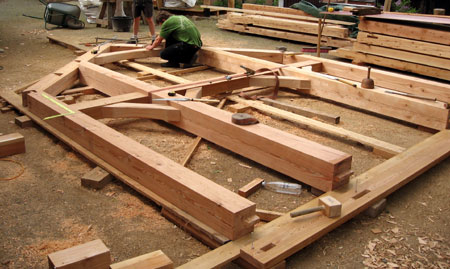
\includegraphics[width=0.99\textwidth]{images/01/Fachwerk_Abbund.jpg}
    \caption[Example of timber frame components being assembled on the ground]
    {Example of timber frame components being assembled on the ground \\
        \footnotesize{(Credits: CC AS 4.0 Licence photo by Georg Hefter - Traditionelles Fachwerk und Timberframe im Vergleich auf georghefter.de)}}
    \label{fig:example-timber-frame-on-ground}
\end{figure}

\subsubsection{Post and Beam Structure}
\label{subsubsection:introduction-post-and-beam-structure}

The third defining characteristic of timber frame construction is post-and-beam structural framing \parencite{jacksobonHistoricAmericanTimber2014,sobonTimberFrameConstruction1984}. The use of large timber sizes in timber frame structures allows them to be strong enough without the use of continuous load-bearing walls. The main benefit is the flexible arrangement of floors and walls to suit different architectural programmes. 
On the other hand, integral timber joints are generally weak in rotational stiffness, causing the joints to behave kinematically. Therefore, diagonal bracing is often introduced to fully or partially triangulate the structure to improve structural stiffness. Being limited by the joint design, these bracings function primarily in compression. It is, therefore, common to design the bracings in complementary pairs to resist dynamic wind loads coming from opposing directions. While some architectural designs may find the intrusion of diagonal bracings obtrusive to usable space, these diagonal bracings are highlighted on the facade as ornamentation in half timber designs \parencite{gernerFachwerkEntwicklungGefuege1979}. In this thesis, the demonstration structures are designed with similar structural principles, specifically the use of structural triangulation in the design offered unique stability advantages during the robotic construction process \seeref{subsection:exploration-4-deformation-awareness-and-error-correction-by-triangulation} \seeref{subsubsection:exploration-4-global-correction-approach}.

Figure \ref{fig:half-timber-frame-example} shows an example of a half-timber style timber frame house in Soest, Germany. Notice the exposed diagonal elements on the facade.

\begin{figure}
    \centering
    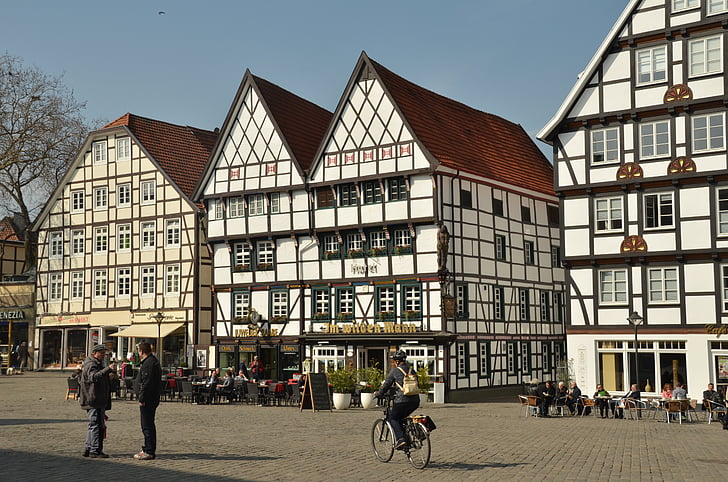
\includegraphics[width=0.99\textwidth]{images/01/germany-soest-architecture-timber-framed-preview.jpg}
    \caption[Example of a half-timber style timber frame house]
    {Example of a half-timber style timber frame house \\
        \footnotesize{(Credits: Licence-free photo, retrieved from \url{https://www.hippopx.com/en/germany-soest-architecture-timber-framed-half-timbered-house-square-city-402214} , n.d.)}}
    \label{fig:half-timber-frame-example}
\end{figure}


    
\subsection{Current Practice of Timber Frame Construction}
\label{subsection:introduction-current-practice-of-timber-frame-construction}

Timber frame construction was once the dominant building method, but it gradually declined in popularity during the 19\textsuperscript{th} and 20\textsuperscript{th} centuries. The advent of industrialization and mass production led to the availability of cheaper building materials such as steel and concrete, which were faster and easier to use. Even within the timber construction sector, newer construction methods that use dimensioned lumber, glulam, LVL, and Cross Laminated Timber (CLT) have replaced timber frame construction. However, in recent years, as more people are aware of the environmental benefits of wood construction, interest in timber frame construction is increasing again as an alternative way to construct with timber. 

Advancements in engineering and design, as well as increased availability of sustainably sourced timber, have helped to make timber frame construction a more viable option for modern building projects. Timber frame components can be prefabricated off-site, which can reduce construction time and costs while also minimising waste and environmental impact. The use of dry-fitted integral timber joints reduces the number of fasteners and components involved, meaning less metal consumption and quicker installation on-site. Furthermore, timber frame structures can be aesthetically pleasing as they often expose the beautiful timber material and reveal the structural load paths. When the joint details are exposed, they can evoke a feeling of tradition and craftsmanship and are often well-appreciated by those who inhabit the building.

\subsubsection{Automatic Machining of Timber Joints}
\label{subsubsection:introduction-automatic-machining-of-timber-joints}

Between the years of decline and its recent resurgence, a number of technological improvements have made timber frame construction more efficient and competitive. One of the major advancements has been the use of automatic joinery machines for carving integral timber joints. Traditionally crafted with hand tools, these joints were labour-intensive and required highly skilled craftsmen that could work precisely.\footnote{The task of marking and setting out was considered the most critical and is often performed by the master carpenter. Other carpenters would prepare materials and carve joints using hand tools such as saws, planes, chisels, and drills.}
Since the invention of automatic joinery machines, the production of timber joints has become highly automatic \parencite{hanshundeggeragCorporateDevelopment2023}. These machines often feature interchangeable cutting tools and can create many types of joints at the beam ends and along its length. Today, the machining of timber joints is very mature and efficient. The automatic joinery machines are controlled by Computer Numeric Control (CNC) technology and can follow a digital program to create timber joints of different designs at different positions. The program can be quickly changed to create different timber elements used for an entire building. \seeref{subsection:introduction-programming-digital-fabrication-machines}

This thesis capitalises on the accuracy and prefabrication efficiency provided by the automatic joinery machines. Accurate parts are highly advantageous for robotic automatic assembly because they ensure accurate manipulation and precise integration. By using prefabricated timber parts with accurately machined integral timber joints, this thesis aims to create a highly automated assembly process, reducing the manual labour needed for adjustment and adaptation. 

\subsubsection{Assembly by Carpenters}
\label{subsubsection:introduction-assembly-by-carpenters}

Although the production of timber frame components is automated, the assembly of the structure is still predominantly manual \parencite{willmannNewParadigmsAutomatic2016}. It usually takes a team of carpenters to assemble a timber structure.

Timber frame structures are almost always assembled on-site due to the nature of their post-and-beam structural system, which favours long and unbroken elements. This means that pre-assembling multiple elements off-site, is not practical because it will result in assemblies that are too big for transportation. 

Below is a summary of the tasks that carpenters perform during the assembly of a timber frame structure, focusing on the structural elements:

\begin{itemize}
	\item \textbf{Sorting timber parts --} Prefabricated timber parts are typically delivered on-site in bundles that correspond to different assembly stages. Many of the components are geometrically unique because of the layout of the joints. Carpenters must identify the correct location for each element based on label and markings on the parts and sort them according to the assembly sequence.

	\item \textbf{Manipulating timber parts spatially --} Post, beam and diagonal bracings are assembled in different spatial (3D) orientations. Carpenters must identify and orient the parts correctly when bringing them to their assembly location.

	\item \textbf{Applying forces --} Because of contact friction and deformation, carpenters may need to apply force to the joints using hand tools. They may use common generic tools such as mallets and screwdrivers (pulling with a screw), or specialise tools such as ratcheting joint pullers. 

	\item \textbf{Aligning mating joints --} Multiple carpenters are often required at every mating joint. They may have to push or pull the already-assembled elements for alignment. 

	\item \textbf{Synchronous Assembly --} During the closure of the joints, the carpenters also ensure parallel and synchronous motion to avoid jamming.

	\item \textbf{Adjusting timber joints --} If a timber part does not fit. Carpenters can remove material or shim gaps. These types of problems are rare with CNC fabricated parts, but can sometimes occur due to poor machining tolerance, design error, machine-programming error, and shrinkage or expansion after machining.

	\item \textbf{Placing fasteners --} Some contemporary joint designs include screws, nails, or dowels.

\end{itemize}

These tasks are the focus of the automated assembly process pursued in this thesis. The challenges of each task are analysed and presented in the next chapter \seeref{section:challenges-mechanical-challenges}.

\subsection{New Opportunities for Timber Frame Construction}
\label{subsection:introduction-new-opportunities-for-timber-frame-construction}

Compared to other newly developed construction methods with a higher degree of prefabrication, the on-site timber frame construction is less economically competitive. For example, modular floor and wall construction allow more components to be assembled off-site (e.g. insulation, windows, doors), which reduces the time and cost associated with on-site work. Volumetric prefabrication (e.g. modular timber construction), which pre-assembled an entire room, further allows the installation of wiring, plumbing, and interior finishes in a factory \parencite{adelDesignRoboticallyFabricated2018}. 

Despite the lack of prefabrication advantages, timber frame construction enjoys greater design freedom because there are fewer transportation constraints when moving linear timber elements than moving a preassembled room-sized timber module. This freedom is essential in creating large-span structures or shell structures where sub-assemblies cannot be effectively transported. In addition, latest timber frame designs have already been able to integrate contemporary building requirements such as plumbing, electrical wiring and insulation that meets building codes \parencite{bensonTimberframeHomeDesign1988}. Therefore, the exploration of automatic assembly for timber frame structures could potentially keep these benefits without the associated penalty of on-site manual work.

\section{Architectural Design to Production}
\label{section:introduction-architectural-design-to-production}

In recent years, the fields of architecture and construction have seen a growing interest in automating various stages of the design and production process. This trend is being driven by the potential benefits of automation, which include increased efficiency, higher precision, and improved quality control. Automation can also help to reduce labour costs, minimise waste, and improve safety on construction sites. While automation has already become common in the manufacturing industry, its adoption in architecture and construction has been slower due to the unique challenges and complexities in the construction sector. Most commercialised examples are limited to prefabrication of small or planar architectural components while only a handful of research projects have attempted to use robotics for structural scale spatial assembly. Therefore, this thesis aims to expand knowledge in this area, starting with the assembly of timber frame structures.

This section will present a brief history of how the timber construction industry transitioned towards digital design and automated production, leading to the current state of the art practices. It is an important starting point to understand whether the assembly process will also undergo such a transition. 

\subsection{Automation from Manufacturing to Construction}
\label{subsection:introduction-automation-from-manufacturing-to-construction}

The beginning of automation started with the manufacturing industry. It involves the use of machinery or computer systems to perform tasks that would otherwise be done by human labour. Without going into details, it typically involves the use of sensors, actuators and control systems to reduce or eliminate the need for human intervention \parencite{nofSpringerHandbookAutomation2009}. It has become a widely adopted practice in the manufacturing industry due to its benefits such as increased efficiency, improved quality, and reduced costs. With automation, the production process can run continuously with a predictable production schedule.

The successful implementation of automation is closely tied to the design and operation of production machines. Since the beginning of industrial automation, automatic machines have undergone several evolutions that are characterised by their features, modes of operations and benefits. Early automatic machines were mechanical systems that performed repetitive fixed operations. Their motions were often defined mechanically through the use of components such as linkages, cams and conveyor belts. Because of this, their motions cannot be easily modified without changing parts. These machines favour high-volume, low variability products that represent the mass-production paradigm of Industry 2.0\footnote{The First Industrial Revolution, aka. Industry 1.0, began in the late 18th century where mass production was carried out by machines powered by water and steam.}.
While some of the earlier machines still require an operator, later machines would contain control systems that are capable of performing cyclic actions on their own. After the introduction of electricity, the use of logic controllers became more common and allowed the machines to make decisions using sensors and signals. The increased level of autonomy allowed further reduction of operator interventions. This type of automation is a typical defining characteristic of Industry 3.0 \parencite{mengesNewCyberPhysicalMaking2015,yinEvolutionProductionSystems2018}. 

Invented in the 1950s and popularised in the 1960s, Computer Numeric Control (CNC) technology further increased the flexibility of machines, such as the aforementioned automatic joinery machines and industrial robotic arms. The motion of CNC machines are defined through the use of a digital ‘program’ such that their motion can be easily modified when products are changed \parencite{wardAutomaticProgrammingNumerically1959}. This is often achieved by incorporating a computerised digital control. The ability to change design quickly eventually led to the mass-customisation paradigm of Industry 4.0. In extreme cases, products can even be unique from piece to piece, resulting in the ‘batch size of one’ paradigm \parencite{wardAutomaticProgrammingNumerically1959}.

The adoption of automatic machines has changed the nature of work from labourers to operators and increasingly towards engineers and programmers \parencite{nobleForcesProductionSocial1986}. While this shift may be difficult for workers unable to acquire a new skill set, it improves the general labour working conditions in the longer term \parencite{stromquistWorldDevelopmentReport2019}. For example, by reducing repetitive manual tasks or avoiding working in dangerous environments. 

\paragraph{A Factory for Making Buildings}

\label{subsubsection:introduction-a-factory-for-making-buildings}

At a larger scale, the concept of automation can be applied to connect different machines together to autonomously regulate production flow. There are two types of connections involved, the first is physical connections, such as using conveyor belts and robotic arms to move parts between machines. The second is logical connections, such as programmable logic controllers forming complex logic networks. In extreme cases, the term \textit{lights-out factory} or \textit{automatic factory} was used to describe large production facilities that are able to sustain continuous production with very few or infrequent operator involvements \parencite{nobleForcesProductionSocial1986,walkerAutomaticFactoryCase1957}. 

Recently, the introduction of large-scale concrete 3D printing technology has brought the automatic factory vision within reach for the architecture and construction community \parencite{ngoAdditiveManufacturing3D2018}. While large-scale 3D printing processes are still at the research stage, smaller 3D printers have already achieved full autonomy, allowing users to press a start button and come back later for the completed parts. The idea of a black-box fabrication machine where design information and raw materials are the only input, was hypothesised to be the future mode of production that can make almost anything \parencite{gershenfeldHowMakeAlmost2012, gershenfeldInternetThings2004}.  

Started in the late 1970s, Japan’s large construction contractors have begun developing robots capable of performing construction tasks. The initial robots were single-task construction robots, designed to perform one specific function, such as finishing concrete, welding, or spray painting \parencite{potterJapanSkyscraperFactories2022}. Starting in the mid-1980s, Japan’s construction robot development shifted away from individual robots, and towards creating an entire robotic construction site \parencite{maedaCurrentResearchDevelopment2005}. The process often makes use of a high number of prefabricated components and focuses on improving the speed for the assembly task. Studies have found that the productivity gain is often apparent when constructing a tall and repetitive building \parencite{linnerAutomatedRoboticConstruction2013,potterJapanSkyscraperFactories2022}. 

While the automated systems seen in Japan are mostly designed for steel and reinforced concrete structures, this thesis studies what it would take for timber construction to achieve a similar level of automation. 

\subsection{Automatic Assembly in Timber Construction}
\label{subsection:introduction-automatic-assembly-in-timber-construction}

In recent years, interest in exploring automatic assembly for timber construction has grown. This was driven by the potential for increased efficiency, precision, and sustainability. Despite the advancements in fabrication techniques, particularly with the advent of CNC technology, the assembly process still presents challenges that industry professionals and researchers are working to address \parencite{willmannNewParadigmsAutomatic2016}.

In the industry, the advancement was mainly focused on the assembly of flat-stackable prefabricated parts, such as light-framed timber floors and walls. Companies like Biesse, Homag, and Weinmann have been developing advanced machinery and automated solutions for timber processing and assembly \parencite{kooTechnologyGapsAchieve2021}. These systems are often large-scale installations similar to a manufacturing production line and are custom engineered for a specific factory. The entire system can include separate material processing stations, such as cutting and joinery machines and for linear timber and panel saws for sheet materials. Processed materials would merge into a central assembly line and be assembled using nails, screws and adhesive depending on its design. Additionally, companies like MiTek and Randek have been focusing on the prefabricated housing sector, developing automated systems for the assembly of timber roof trusses \parencite{ianharveyRoboticArmsAI2018}. 

Despite these groundbreaking efforts, the challenges for spatial timber assembly is rather unique \seerefii{section:challenges-mechanical-challenges}{section:challenges-computational-and-design-challenges}. These challenges are complex, interdiscipline and are often specific to the construction system. This makes it hard to generalise solutions between different type of constructions. For example, despite having high demand in the industry, the spatial assembly of planar walls to create volumetric timber modules is still performed manually; timber frame structures, despite existing for a long time, still have no automatic assembly solutions. As the demand for sustainable building solutions continues to grow, and the skilled labour market continues to shrink, the exploration of automatic assembly methods for timber construction is urgently needed. 

Several innovative research projects have emerged in recent years, addressing the challenges of spatial manipulation of linear timber elements. For instance, the pioneering work conducted by Gramazio Kohler Research at ETH Zurich has shown the potential of using industrial robots to assemble complex timber structures. While early explorations were limited to a 2.5D stacked assembly approach \parencite{apolinarskaSequentialRoof2016, gramaziokohlerresearchethzurichStackedPavilion2009, helmInSituFabricationMobile2014}, many later projects addressed 3D spatial manipulation. For example, the first two-story robotically assembled structure \parencite{eversmannRoboticPrefabricationTimber2017}, the volumetric timber modules of the DFAB House \parencite{adelDesignRoboticallyFabricated2018, thomaRoboticFabricationBespoke2018}, and many other spatially assembled timber structures \parencite{apolinarskaRoboticAssemblyTimber2021, eversmannRoboticPrefabricationTimber2017, helmAdditiveRoboticFabrication2016, helmreichRoboticAssemblyModular2022,willmannNewParadigmsAutomatic2016}. Similarly, other research institutes have demonstrated the capabilities of using industrial robots to assemble prefabricated timber plates spatially \parencite{robellerRoboticIntegralAttachment2017, rogeauRoboticAssemblyIntegrallyAttached2023} and to assemble modular timber cassette systems \parencite{alvarezBUGAWoodPavilion2019, claypoolAutomationDiscreteExploring2021}.

This thesis aims to contribute to the ongoing efforts to advance the state of the art in this domain. Using timber frame construction as a starting point, the assembly problems are studied and addressed in a holistic way, with the intention to improve the understanding of these problems and for generalizable solutions to emerge.

\subsection{From Automation to Digital Fabrication}
\label{subsection:introduction-from-automation-to-digital-fabrication}

In the 1990s, various computer programmes that were intended for animation (e.g. Alias Wavefront, Maya) and engineering (e.g. Catia, later DigitalProject) were adopted by the architectural community for modelling geometrically complex buildings. This partially triggered the bloom of freeform architectural designs that are made famous by architects such as Frank Gehry, Zaha Hadid, Santiago Calatrava. For example, \textit{Fishdance Restaurant, Kobe (1989),  Guggenheim Museum Bilbao (1997), Walt Disney Concert Hall (2003)},and \textit{ Louis Vuitton Fondation (2014)}.\textit{ }

The immediate implication of freeform architectural designs is the need to produce geometrically complex components. This was addressed by the use of CNC machines that can follow arbitrarily complex paths. However, freeform architectural designs also implies the need to produce a large amount of non-repetitive components. At the component level, this is similar to the mass-customisation paradigm in manufacturing. However, in order to create the unique CNC programmes for the production process, Computer-aided design (CAD) and computer-aided manufacturing (CAM) software became an indispensable part of the production workflow \parencite{sheldenDigitalSurfaceRepresentation2002}. 

\textit{CAD software} allows architects and construction engineers to create 2D or 3D models of buildings, including the detailed geometry of each building component. Using these models, production engineers use \textit{CAM software} to generate toolpaths for the CNC machines. Because of the non-repetitive geometry, each component requires a unique programme for the CNC machines for operation and unique drawings for the workers to perform the assembly and inspection. This eventually leads to a workflow where not only are the machines automated, but the production of information is also automated. This new mode of production became what is known now as \textit{Digital Fabrication}.

The basic workflow for CAD is called direct modelling, where designers explicitly create and modify geometry in a linear workflow. This can be analogous to the ‘drawing’ process in architectural design as the designer interacts with the computer program over a graphical user interface (GUI) in an interactive way. The designer can use functions offered by the CAD to add or modify geometry. A more advanced workflow is \textit{parametric modelling}, where the history of modelling operation is saved for later reuse. This can be as simple as a ``Macro", where multiple functions are chained for easy access, or as complex as to define geometry based on a chain of functions and input parameters. This can be analogous to writing a mathematical equation with functions and variables. By changing the input values to the variables, the equation can be used to represent many possible outcomes. Therefore the output of a parametric model is dynamic and can be regenerated if necessary. Designers typically create a parametric model in one of the two ways. The first method is by demonstrating the modelling or computation logic to the CAD programme while the programme ‘records’ the logic which can be reused later. The second method is to create a symbolic description, similar to computer programming. This is often called \textit{Scripting} and is often used for more complex logic. Depending on the CAD programme, this symbolic script can be written in one of the many programming languages (e.g. C$\#$, Python) or, more recently, in a graphical programming interface (e.g. Grasshopper, Dynamo). 

There are two important benefits of a \textit{reusable CAD workflow}. The first is to save time when modelling large amounts of geometrically similar (but not identical) parts. The second benefit is the ease of making design changes. For example, the designer only needs to change the inputs for the CAD programmes to update the downstream documents automatically. These can include 3D models of components, 2D drawings and assembly instructions. In recent years, the popularity of parametric workflow has shaped the way designers interact with the design process. Instead of focusing on the final outcome, the automated workflows allow them to design the geometrical logic first before adjusting the input parameters to achieve the desired geometry \parencite{jabiParametricDesignArchitecture2013}. In addition, measurement and evaluation logic can also be incorporated into the script, allowing designers to be more informed about their designs. Complex relationships between geometry and structure can also be scripted to allow an intuitive and interactive design process \parencite{pottmannArchitecturalGeometry2007, woodburyElementsParametricDesign2010}. This design process that is supported by parametric modelling is often called \textit{Parametric Design}.

\subsection{Programming Digital Fabrication Machines}
\label{subsection:introduction-programming-digital-fabrication-machines}

Reusable workflows have also been extended to the CAM software to generate machining programmes automatically. This refers not only to the automated creation of toolpaths from a part geometry, but also the automatic decision-making to choose machining strategy, tool choice, machining sequence, and machining speeds. In the architectural context, this type of workflow has been used for cutting 1D profile materials and 2D sheet materials for geometrically complex facade systems used in free-form buildings \parencite{eigensatzPanelingArchitecturalFreeform2010, sheldenDigitalSurfaceRepresentation2002}.

In timber construction, the aforementioned automatic joinery machines were invented before the digital fabrication revolution \parencite{hanshundeggeragCorporateDevelopment2023}. Programming work for these machines was initially done by manually entering joint parameters (such as joint type, size and location on the beam). However, this work was soon automated by CAD (e.g. Cadwork 1988) and CAM (e.g. LignoCAM) software that was developed for the timber industry \parencite{schwinnManufacturingPerspectives2016}. Timber-specific CAD software improved efficiency for modelling matching pairs of joints across different elements and reduced the risk of design errors. While the CAM software is responsible for converting the joint features of the 3D model (such as cutouts and drill holes) into machine-specific programmes for the automatic joinery machines.

In the early days, CAD and CAM functionality were integrated into the same programme. However, as more machine manufacturers such as Biesse, SMC Group, and Homag started to make automatic joinery machines, open file formats were developed to allow different CAD, CAM and automatic joinery machines to work interchangeably. The current industry standard is the BTL (2006) and later BTLx (2015) format for data exchange. They were developed by a collaborative effort from the industry to create a specialised format for describing timber components. For example, it can represent timber grain directions, glulam orientation and joint machining tolerance that would otherwise not be possible using generic 3D model formats \parencite{lignocamBTLxWhatIt2020, design2machineHistoryDataTransfer2023}. 

The design-to-production workflow would typically start with a timber engineer that creates 3D models of the arrangement of beams and joints in the CAD software. Design iterations would happen within the CAD programme until architectural and structural requirements are met. Construction planning would also be performed in the CAD environment for specifying the production schedule and assembly sequence. The description of the beams and joints would then be passed to machine-specific CAM software by using, for example, the BTLx file format. The CAM programme would be able to recognise the timber elements and their joint details and make machining decisions specific to the fabrication machine setup. For example, to choose a suitable saw, mill bit or drill bit size from a collection of available tools; or to decide whether a hole is drilled or milled.

A production engineer, who has intimate knowledge of the machine setup, is often involved in defining the rules that the CAM software would follow. The ruleset would include a description of machine limitations, available tools, material choice, desired machining quality and production sequence. Conceptually, this is similar to the reusable CAM workflow mentioned above with a similar intention to automate the CAM software, to handle a large number of geometrically unique elements. 

Hypothetically, the assembly process studied in this thesis can also adopt a similar workflow. There is a strong similarity between creating machining programmes and creating robotic assembly programmes. Both of them are specific to the machine setup (e.g. robot kinematics), machine limitation (e.g. avoiding collisions) and tools setup (e.g. end effectors). It also needs to overcome the complexity of making decisions according to unique geometry. Therefore, this thesis adopts the parametric modelling and reusable workflow from machining as a starting point and apply it to robotic timber assembly \seeref{subsection:exploration-3-workflow-for-generating-assembly-programmes}. 

\subsection{Fabrication-aware Design}
\label{subsection:introduction-fabrication-aware-design}

\begin{quote}
	``While digital models are easily created, the actual fabrication and construction remain a challenge.'' \parencite{pottmannArchitecturalGeometryFabricationAware2013}
\end{quote}

The disconnection between design and fabrication is the source of numerous frustration that forced many geometrically complex projects into a ‘redesign’ phase after the reality of fabrication and construction limitations was imposed. This redesign process is known as rationalisation \parencite{pottmannArchitecturalGeometryFabricationAware2013}. A rationalisation is a design negotiation between keeping the design intent and reducing fabrication costs. It invariably led to a loss of fidelity. A better approach would be to incorporate knowledge of the actual construction process during the design stage; this is known as construction-aware or fabrication-aware design.

In the current architecture and construction industry, the role of evaluating constructability lies in the hand of a construction engineer. Very often it is a single-direction workflow that is difficult to accommodate frequent design changes. As architectural design practices migrate towards a digital workflow, there is a growing interest to automate the evaluation process. One common approach is to encode the knowledge of the fabrication constraints as computational algorithms, which can be computed automatically within the CAD design software. Feedback can therefore be provided as quickly as possible for the designers, which gives them a better chance of pushing designs closer to fabrication limits yet without violating them. 

These automatic checks, also known as design validation, are particularly useful when dealing with designs that have many unique parts (that would otherwise need to be checked individually) or when the fabrication limitations are complex or obscure. They also help avoid human errors and mistakes that are costly to fix downstream. 

While the concept of fabrication-aware is often used to check prefabricated components and machining processes, the concept can hypothetically be applied to a robotic assembly process. For example, robot reachability, payload, and collision. As long as a constraint can be modelled as a computable algorithm, it can be checked automatically. However, in practice, not all checks are easy to model and certain behaviour requires advanced simulation to model. This will be further elaborated in the next chapter \seeref{section:challenges-computational-and-design-challenges}. However, it is exactly because of this complexity that makes it difficult for a designer to evaluate them manually. Therefore in the context of this thesis, one of the main explorations is to study whether robotic assembly processes can be checked automatically and whether a fabrication-aware design workflow is feasible. 

The following sections present two case studies in the field of digital fabrication. They provided a positive indication that an integrated design and fabrication workflow is achievable.

\subsubsection{Case Study - Automatic CNC Machining Programme}
\label{subsubsection:introduction-case-study-automatic-cnc-machining-programme}

The first case study is a comparison between robotic assembly and machining processes. Assembly robots are similar to complex milling machines with multiple axes in the sense that they are both capable of making complex movements. However, they are also prone to programming errors that can cause expensive damage. Therefore, when creating toolpaths, a CNC programmer will often rely on the multitude of checking algorithms offered by the CAM software to catch potential problems. It is common for a CNC programmer to resolve production problems separately, within the scope of modifying machine parameters, tooling or cutting strategy. It is only until the attempts are exhausted that the programmer will suggest design changes to the designer. 

The culprit of this long evaluation cycle is that the current practice of creating toolpaths requires a lot of manual input. On the one hand, this offers many optimization possibilities for the machining process but at the same time makes feasibility evaluation very complex. In order to address this problem, researchers have identified the need to combine the automatic generation of toolpaths and automatic validation \parencite{garciaProcessPlanningBased2011,sheenMachiningFeatureRecognition2006, joshiGraphbasedHeuristicsRecognition1988}. These methods have already been adopted by companies offering machining services to generate CNC programmes automatically. This enabled them to provide almost-instant price quotations for parts solely based on a geometrical model. 

Similar to the hypothesis proposed before \seeref{subsection:introduction-programming-digital-fabrication-machines}, there are a lot of similarities between an assembly process and a machining process. Perhaps the same automatic generation and validation principle can be applied to robotic assembly processes to enable a more integrated workflow.


\subsubsection{Case Study - Automatic Slicing for 3D Printing}
\label{subsubsection:introduction-case-study-automatic-slicing-for-3d-printing}

Another parallel can be drawn between robotic assembly and additive manufacturing. Fused Deposition Modeling (FDM) Printers are mechanically simple devices that can create 3D parts by stacking 2D slices. However, the generation of toolpaths (a.k.a slicing) requires advanced algorithms to determine optimal toolpath, layer height, infill density, print speed, and other settings based on the geometry of the model, the type of printer, and the material being used. Additionally, the slicer software needs to take into account various non-linear factors that can affect the quality of the printed object, such as the cooling rate of the material, the shrinkage of the material as it cools, and the adhesion of the material to the print bed. Slicers may also include features such as support generation, which creates structures to support overhanging features of the model during printing. 

As a result, slicers can be quite complex and require a significant amount of tuning and customization. Nevertheless, pre-tuned slicers for commercially available printers can produce satisfactory results for almost any 3D geometry. In many cases, they are fully automatic upon the reception of a CAD model and do not require any manual input. When processing a problematic design, such as large overhangs, the software is able to pinpoint the problematic area for the designer to resolve. 

Similarly, robotic assembly processes also require complex software algorithms to model robot kinematics, tool behaviour, and environmental limitations. The fact that full automation can be achieved in slicer programs provides an optimistic indication that robotic assembly processes may achieve a similar degree of automation.

\section{Robotics in Architectural Assembly}
\label{section:introduction-robotics-in-architectural-assembly}

Robotics involves various disciplines that deal with the design, construction, operation, and use of industrial robots. The disciplines include mechanical engineering, electrical engineering, and computer science. Industrial robots play a crucial role in performing tasks autonomously or with minimal human intervention. There are many types of industrial robots, typically classified by their kinematic configurations, such as Cartesian Robots, Cylindrical Robots, and Articulated Robots \parencite{waldronKinematics2016}. Articulated robots, also known as robotic arms, are the most common type used for spatial manipulation. They typically contain 4 to 7 rotary joints (usually 6) arranged in a chain and connected by rigid metallic bodies. This allows spatial positioning and agile movements beyond orthogonal directions.

Robotic arms are multipurpose machines that can be used for material handling, machine tending, and performing assembly tasks when equipped with a task-specific tool. This tool is known as an end-effector. In the context of this thesis, the assembly task is the size of a building. In order to extend the reachable area of a robotic arm to cover the entire volume of the construction, a unique setup is used where a robotic arm is mounted inside a 3-axis overhead gantry\seeref{subsection:methodology-laboratory-context}, a configuration similar to the Japanese building factories.

Many research projects have already explored the adaptation of robotic arms to perform architectural assembly tasks \seeref{subsection:introduction-automatic-assembly-in-timber-construction}. However, the use of robotic arms in the construction industry presents unique challenges due to the non-repetitive nature of the tasks involved. The two main challenges relevant to this thesis are the inaccuracy of non-repetitive targets and the automation of planning non-repetitive trajectories.

\subsection{Inaccuracy for non-repetitive targets}
\label{subsection:introduction-inaccuracy-for-non-repetitive-targets}

Most of the industrial robotic arms available in the market today were designed for the manufacturing industry. Their long kinematic chains are designed to be able to reach into tight spaces such as machine openings and car interiors. For this purpose, agile motions are preferred over mechanical stiffness and accuracy. In the context of manufacturing, robotic tasks are often repetitive, targets and payload are also known in advance during programming. As long as the robot repeatability is good, manual calibration can be performed to achieve good alignment, this is known as Teaching \seeref{subsection:exploration-3-robot-targets-taught-configuration-and-cartesian-pose} \parencite{shohamRobotTeachingMethods1984}.

However, the difference between repeatability and accuracy is important to consider when using robotic arms for non-repetitive tasks. Repeatability refers to the robot's ability to return to a specific position with high precision, while accuracy is a measurement of the robot's ability to reach a previously uncalibrated target position. This is much more challenging for the robot to achieve because it needs to take into account discrepancies in the robot kinematics model, manufacturing tolerance of the robot parts, and deformation of the robot under different payloads and configurations. 

While the kinematic model of a robot can be calibrated \parencite{mooringFundamentalsManipulatorCalibration1991}, the changing deformation due to payload and configuration is hard to predict. Formally, this is the difference between open-loop (repeatability) and close-loop (accuracy) control concerning the end-effector poses. At the moment, most of the industrial robots on the market (including the one used in this thesis) are only close-loop controlled until the joint positions. The end-effector pose is open-loop controlled.  

Using robotic arms for architectural assembly typically entails a large number of unique targets. However, manually teaching each unique target would defeat the purpose of automation. Therefore, the practical limitation of this inaccuracy is studied in this thesis. For example, how it affects the timber frame assembly process, what are the associated failure modes, how does it affect failure rate and what strategies can be used to mitigate the problem. For the sake of clarity, it should also be pointed out that redesigning a robotic arm is beyond the scope of this thesis.

\subsection{Automation for planning non-repetitive trajectories}
\label{subsection:introduction-automation-for-planning-non-repetitive-trajectories}

The anatomy of a robot program can be seen as a segment of movements that goes from one target to the next. The trajectory is simply a matter of interpolating between different targets. However in reality, there are many limitations to this interpolation. For example, some robotic joints cannot be rotated through 360 degrees between interpolation, or if the interpolation results in a collision.

In industrial automation, the production engineer will typically teach waypoints for the robot to move around obstacles. Once the teaching is completed, the engineer will also verify the motion at a slow speed to ensure it is collision-free and later at higher speed (production speed) to ensure dynamic effects are acceptable. Although this process of teaching and validation is tedious and time-consuming, it is acceptable for a repetitive process, because it has to be done only once. 

Alternatively, the configurations and associated trajectories can also be created in a computer simulation, using algorithms that are referred to as motion planners\parencite{lavallePlanningAlgorithms2006}. This workflow requires all the objects and machines around the robot being modelled in the simulated environment for collision checking \seeref{subsection:exploration-2-motion-planning}. Even so, small adjustments may be required in the physical environment as the alignment between physical setups and their simulated counterpart may differ significantly.

For planning non-repetitive trajectories the impracticality of teaching the targets means that simulated motion planning must be used. Therefore it will suffer from the accuracy problem when alignment is needed with real world objects. Moreover, the construction environment must be accurately modelled and cannot be changed during the robot operations. 

% \chapter{Discussion}
\label{chapter:discussion}

This thesis started with the aim of exploring the automatic assembly of timber frame structures with industrial robotic arms. However, as the investigation progressed, unforeseen discoveries and the development of the Distributed Robotic Tool (DiRT) concept, prompted a shift in the research focus. The new findings expanded the scope of the study, going beyond the initial research questions that guided its early stages. Consequently, the original questions were augmented to address the emerging knowledge gaps, reflecting the dynamic and evolving nature of the research.

In the preceding chapters, I have presented the validation experiments, observations, and lessons learned in each development iteration, following the chronological order of their discovery. In this Discussion chapter, I will analyse the results with a focus on understanding recurring patterns, providing generalisable theories, and discussing implications. I will start by responding to the original research questions posed at the outset of the dissertation before expanding into other topics that extend beyond them. This expansion reflects my commitment to exploring the most pressing issues within the domain of construction robotics. Finally, I discuss the potential for the versatile Distributed Robotic Tool (DiRT) concept to be adapted for use in other construction systems beyond timber frame structures,

It is important to note that much of the reasoning and conclusions in this chapter are based on the observations presented in earlier chapters. Links to those sections will be provided where appropriate to avoid repetition, but readers are advised to read the development chapters first for a comprehensive understanding.

Additionally, readers should be aware that the inductive approach used to explain observations in this chapter is subjective and interpretive in nature. The aim is not to prove or disprove a hypothesis but to find meaning through observations, to formulate new problems, to clarify concepts, and to form new hypotheses.

\section{Response to Research Questions}
\label{section:discussion-response-to-research-questions}

	\paragraph{1. What technologies are required to assemble time frame structures?}

The DiRT system developed in this thesis demonstrated a viable method to overcome the challenges of assembling timber frame structures outlined in the introduction \seeref{chapter:challenges-and-research-goals}. In particular, the use of modular assembly tools to apply high forces to the joints proved to be a reliable solution for overcoming misalignment \seeref{subsection:challenges-joint-alignment} and high assembly resistance \seerefiii{subsection:challenges-sliding-friction}{subsection:challenges-tight-fitting-joints}{subsection:exploration-2-clamping-joints-with-chamfered-edges}. The flexibility to attach tools where needed allows the system to assemble many types of structures with different joint types, jointing angles, and timber sizes, with and without fasteners. In addition, the local correction effect at each joint was found to be exploitable for preventing global error accumulation.

\paragraph{2. What are the robotic end effectors needed to assemble the joints?}

The DiRT concept introduced a significant change to the traditional definition of robotic end-effectors, transforming them into hybrids that incorporate elements traditionally found in mobile robots, such as embedded controllers, batteries and wireless communication. The modular nature of these tools enables various implementations based on specific joint requirements. In this thesis, two families of assembly tools were designed for a variety of lap joints \seerefiii{subsection:exploration-2-parametric-variations-of-lap-joints}{subsection:exploration-4-parametric-polyline-lap-joints}{subsection:exploration-4-parametric-non-planar-lap-joints}. One closes a joint by clamping it from the outside \seeref{subsection:exploration-2-lap-clamp-cl3-hardware}, while the other tightens a screw through the joint's centre \seeref{subsection:exploration-4-sl1-screwdriver-electronics}. The different placement options of the two tools also showcase the flexibility of attaching the DiRT tools either on the robot side or on the stationary side. Both modes of operation are useful depending on the type of joint being assembled.

\paragraph{3. Can the DiRT tools be general-purpose, or are specific to the type of joint being assembled?}

DiRT is a general-purpose concept that can be extended for assembling different types of joints and other structures. In general, large-scale assemblies, especially ones that require multiple joint alignments and closure, can benefit from using DiRT. The only essential component of a DiRT tool is the docking adapter for the robotic arm to manipulate it. 

A DiRT tool does not even have to contain an active actuator. For example, the temporary scaffolding \seeref{subsection:exploration-5-scaffolding-support-during-assembly} used in the CantiBox can be converted to a DiRT tool \seeref{subsection:discussion-designing-new-dirt-tools} for it to be installed robotically.

\paragraph{4. Is the accuracy of a typical industrial robot sufficient to assemble timber beams with joints? Is it necessary to develop sense, alignment and compensation methods to overcome misalignment?}

There are a few types of alignment problems that are relevant to robotic timber frame construction. The first is pairwise alignment between two joints. This requires extreme accuracy because the joints are typically designed to be tight-fitting with no misalignment tolerance. During the development, this is shown to be solvable by the use of high assembly force and chamfered joint edges. Thanks to the low stiffness of timber and the programmable compliance of the robotic arm, the two pairs can be guided into alignment \seeref{subsection:exploration-4-compliant-control-for-robotic-arm}.

The second alignment problem occurs when there are more than one joint being assembled at the same time. The partially-assembled structure can deform in different directions, creating an overconstrained scenario and a conflict among alignment directions for each joint pair. However, what was thought to be a problem turns out to be a beneficial property. Observation shows that the local corrective behaviour at each joint can correct the deformation on the already-assembled structure. This allows the use of strategically designed timber parts to prevent global error accumulation \seeref{subsection:exploration-4-deformation-awareness-and-error-correction-by-triangulation}.

The third alignment problems arise from the use of robotic arms to manipulate DiRT tools. The implementation is challenging because tight tolerance is required to successfully place them on or retrieve them from the partially-built structure. The problem is worsened by the large deformation often seen on the partially-assembled structure. To address this issue, a contactless camera-marker alignment method was developed. The test result shows that it can direct the robotic arm to correct large deviations and achieve good alignment \seeref{subsection:exploration-4-camera-marker-alignment-correction-system}.

In general, it is not possible to answer whether an alignment will be successful. Different alignment scenarios have different amounts of deviation depending on the robot pose, the state of the partial assembly and many other factors that are unique in each moment. The correction mechanisms used, whether passive or active, have different correction ranges and success rates. The complexity of this problem is detailed in \\noseeref{chapter:new-hypothesis}, with a newly developed model to relate the probability of success with predictable deviations.

\paragraph{5. How suitable is an industrial robotic arm for performing spatial timber assembly? How can they be optimised for construction purposes?}

The RFL robotic platform demonstrated sufficient accuracy in assembling the three demonstrators using active and passive alignment correction methods. The kinematic combination of a robotic arm and an overhead gantry effectively manipulated the DiRT tools and timber components spatially to perform the assembly tasks. It provided good reachability to bring long timber elements through small openings of the structure and to attach and detach tools from tight spaces. However, if robots can be designed with longer and slimmer forearms, it could improve reachability and design flexibility. \seerefiii{subsection:exploration-2-robot-collision-problems}{subsection:exploration-2-robot-cables-problems}{subsection:exploration-3-robot-cable-guides}

The overhead clearance provided by the gantry proved beneficial for finding collision-free trajectories during motion planning. This is because the robot carrying long beams can easily traverse the space above the partially-assembled structures. Nonetheless, care is needed to ensure ground-level operations are reachable and executable by the robot \seeref{subsection:exploration-4-beam-to-ground-connection}.

On the downside, these demonstrators have pushed the robotic arm to its payload limit. Given that the demonstrators were small compared to actual buildings, future implementations should address the payload issue for larger structures. While it may not be feasible to increase reachability and payload while keeping a robotic arm slim, operation speed is less critical for construction robots and could potentially be sacrificed to accommodate improvements in other areas.

Lastly, current industrial robotic arms cannot detect and correct deviations caused by body deformation. Due to the non-repetitive nature of construction, robotic repeatability is no longer the only relevant specification. Construction robots need to reach a target pose accurately regardless of configurations, and payloads and to achieve this on the first try \seeref{subsection:new-hypo-accuracy-of-robotic-platforms}. Therefore, future construction robots should consider sensors that can measure body deformation and total flange deviation in real-time. This will allow absolute accuracy beyond repeatability. 

\paragraph{6. How many robots are needed to assemble a building?}

The combination of a single robotic arm and an overhead gantry has proven sufficient for constructing all the demonstration structures. Adding more arms may improve productivity, but the effect may not be easily quantifiable due to the harmful effect of overcrowding the planning scene. Multiple robots in collaboration may also enable tasks that are currently not possible, such as holding long beams at two points, creating sub-assemblies, or providing temporary structural support.

\paragraph{7. How can computational tools support a robotic assembly process?}

Computational tools are essential in supporting robotic assembly processes. In this thesis, their primary function is to assist users in designing the sequence of the assembly process, planning robotic tasks, and visualising, validating, and executing them. 

The modelling method is similar to traditional CAD and CAM software, but includes the concept of a step-by-step assembly process. This allows the user to model the changing location of objects and robots during the assembly. Interactive design and evaluation workflow was found to be useful for designing the robotic process modelling \seeref{subsection:exploration-2-motion-planning}.

The creation of the robotic programme consists of two main steps. The first step is task planning - to create a list of task descriptions that need to be executed. The second step is motion planning - to create robotic trajectories for the robotic motion tasks. These two steps can also be performed together and are known as Task and Motion Planning (TAMP). It is not only a computationally expensive process to search for collision-free robotic motions but also a difficult formulation problem for designers to convert the design of a structure into task descriptions for the computational algorithms to compute. In order to address this, my collaborator YiJiang Huang and I created two different types of formulation methods that bridge the gap between designers and programmers \seerefii{subsubsection:exploration-3-task-planning-with-flowchart}{subsection:exploration-5-specifying-actions-and-goals-for-tamp-with-pddlstream}.

Because TAMP is a stochastic search in a high-dimension space, it is common to set a search limit for the process to decide when to give up. If a solution can be found within the given time, the assembly is considered constructible, and its motions can also be visualised \seeref{subsubsection:exploration-2-mp-as-a-design-feasibility-check}. However, in the context of timber frame construction, the assembly scene is often a congested space that makes it hard for the robot to manipulate long timber beams. It is not uncommon for TAMP to fail even after hours of search \seeref{subsection:exploration-2-narrow-passage-problem}. This creates frustration for designers to wait for long hours only knowing that something went wrong. A better approach is to use lower-fidelity checks that are faster to perform for a more efficient fabrication-aware design workflow. Even if the quality of the check is not perfect, it is good enough to provide early-stage feedback to the designers. \textit{(see \ul{question 9 below})}

\paragraph{8. Can robotic programmes be generated automatically based on assembly design?}

The non-repetitive nature of architectural construction makes process modelling and TAMP a tedious task. Even the assembly of a simple structure involves thousands of steps \seeref{subsubsection:exploration-3-expanding-task-groups}. The sheer number of unique assembly scenes, robot targets, and motion constraints make manual modelling infeasible. Therefore, it is highly desirable if the static model of a timber structure can be automatically converted to robotic programmes.

During the development, it was found that all of the robotic movement targets can be extracted from the design model using rule-based algorithms \seeref{subsubsection:exploration-3-compute-robot-targets}, but some decision related to the robotic process have to be decided by a production engineer \seeref{subsubsection:exploration-3-process-visualization-and-adjustment}. For example, the number of simultaneously assembled joints for a specific beam can be inferred from its joint-neighbour relationship from the design model. The position of that beam before closure can then be inferred from the assembly direction of each of the mating joints. If those joints are clamped, the task list for attaching the clamps can also be inferred from the number of joints, their positions and their required clamp model \seeref{subsubsection:exploration-3-task-planning-with-flowchart}. Unfortunately, these algorithms are problem specific and are likely to require manual redesign when the assembly logic is changed. 

In some cases, the inference rule may contain more than one possibility for a decision, for example, the position where the robot holds a beam. In this thesis, the production engineer made the decision \seeref{subsubsection:exploration-3-process-parameters}. However, it is possible that some rule-based or search-based algorithms can be developed in the future to make these decisions automatically. For example, during the design of the HyparHut and CantiBox, simple rule-based algorithms were tested and have been shown to reduce manual input to minimal. The remaining decisions are likely to be fully automatable if better modelling and automatic checks are developed, such as automatic deviation analysis\seeref{section:estimating-deviations}.

In addition, I have found that the data structure of the static model has a large influence on the difficulty when creating these inference algorithms. For example, how neighbour relations are described, and how beam and joint information is stored \seeref{subsection:exploration-2-assembly-model-data-structure-and-functions}. While a working data structure is developed for the timber assembly problem in this thesis, more work is needed to understand if it can be generalised. 

\paragraph{9. How will design validation be performed?}

Existing timber construction practice is typically concerned with structural validation (at both global and joint level) and Computer Numeric Control (CNC) fabrication validation (to make sure joint details can be machined). While these validations are still required, the added robotic assembly process requires specialised validation to make sure it can be planned and executed. 

Practical experience has shown that some validation checks can be performed during design time with very fast feedback. This include: 

\begin{itemize}
	\item Infeasible assembly direction because of geometrical interlock
	\item Robotic payload limit \seeref{subsection:exploration-4-heavy-beam-caused-robot-overload}
	\item Robotic reachability (IK + CC) \seeref{subsection:exploration-4-fast-design-validation-with-ik-check}
	\item Collision between parts at keyframes
	\item Availability of assembly tools for all mating joints
\end{itemize}

On the other hand, TAMP is a much slower process that cannot provide real-time feedback to the designer. For example, it takes approximately 10 hours to compute TAMP for each demonstrator. The workflow feels like a ‘compile’ process to the designer, similar to the compile process in software development. The designer can only know for certain if the design will be constructible after a long wait \seeref{subsubsection:exploration-2-mp-as-a-design-feasibility-check}. Moreover, due to the highly coupled and linear planning scene, even small design changes necessitate the re-computation of TAMP.

In order to address this, my collaborator and I have discovered different types of validation checks that can be performed, depending on the affordable time. This multiple level-of-detail validation process appears to be a practical approach to evaluating a design. The checks in increasing level of accuracy are:

\begin{itemize}
	\item Collision Check ($<$ 1 minute)

	\item IK + CC (a few minutes) \seeref{subsection:exploration-4-fast-design-validation-with-ik-check}

	\item LMG Planning (10 to 15 minutes) \seeref{subsection:exploration-4-planning-order-by-motion-group}

	\item Motion Planning (a few hours) \seeref{subsection:exploration-3-non-sequential-planning-order}

\end{itemize}

\paragraph{10. What are the design constraints resulting from an automatic assembly process?}

In this thesis, DiRT tools have been developed for lap joints only and therefore the demonstrators are also designed exclusively with lap joints. While there are certain design constraints found during demonstrator design, it is hard to evaluate whether these constraints are caused by the specific tool implementation, the absence of other joint types, or if they represent a fundamental limitation with the DiRT concept itself. Especially because DiRT is an open system and new tools can always be added to solve a specific problem.

The only notable non-generalisable limit of the DiRT concept is the requirement for the tools to be attached to the structure or on the part being assembled. This restricts their attachment points to positions with sufficient stiffness to support the tools \seeref{subsection:exploration-2-unstable-structure-during-assembly}. It is easy to speculate that timber sizes smaller than those used in the demonstrations may struggle to hold the tools in place. Since it is unlikely that the DiRT tools can be made significantly lighter, the assembly process could potentially be scaled up, but scaling down may be challenging.

\paragraph{11. Can joint details be adapted to make automatic assembly easier?}

There are a number of construction details that are used to facilitate automatic assembly. In general they can be grouped into two types based on the intended purposes. The first type of details are for alignment correction, such as the chamfered edges in the lap joint for correcting pairwise alignment, and the fiducial markers added on the timber surfaces for camera vision \seeref{subsection:exploration-4-camera-marker-alignment-correction-system}. The second type of details is used for registration, such as the registration holes machined on the beam that helps alignment with the robotic gripper and for the DiRT tools to be attached correctly \seerefii{subsubsection:exploration-1-gripper-for-hanging-clamp}{subsection:exploration-4-parallel-gripper-pg1500-for-long-beams}.

In general, when designing construction details to facilitate automatic assembly, it is essential to examine whether that detail can be fabricated easily. In the case of timber construction, its compatibility with an automatic joinery machine is essential. In addition, reductive features such as registration holes and chamfered edges may have negative impact on structural performance and should be carefully studied.

\paragraph{12. How will an automated timber construction process be implemented? What are the new domain experts and their responsibilities?}


Considering the significant capital investment required for a large-scale robotic platform, it is essential for a DiRT system to be reusable across multiple projects with minimal modifications. A practical implementation would likely involve the development of an initial system prototype, similar to the one demonstrated in this thesis, which would be progressively improved over time. As the initial system becomes operational, additional DiRT tools, scaffolding elements, and sensors can be incorporated from project to project, thereby expanding the range of joint types and building components that can be assembled.

Based on the experience gained from operating the system, it is possible to speculate on the various domain experts needed during this expansion phase. Generally, some roles would be more focused on generic system design, while others would be responsible for executing projects and making project-specific modifications.

\begin{itemize}
	\item \textbf{System designer (CAD / CAM)}

	\begin{itemize}
		\item Create modelling tools for designers in CAD environment 
		\begin{itemize}

			\item Create parametric models of beams and joints \seeref{subsection:exploration-4-parametric-polyline-lap-joints}

			\item Create design validation algorithms \seeref{subsection:exploration-3-design-software-implementation-in-rhino-python}

		\end{itemize}
		\item Formulate assembly logic as TAMP problems

		\begin{itemize}
			\item Create task planning flowcharts\\
			\seeref{subsubsection:exploration-3-task-planning-with-flowchart}
			\item Create an action-state description for automatic TAMP \seeref{subsection:exploration-5-specifying-actions-and-goals-for-tamp-with-pddlstream}

		\end{itemize}
		\item Create process visualisation and reporting tools for designers, engineers and operators. \seeref{subsubsection:exploration-3-process-visualization-and-adjustment}

	\end{itemize}
	\item \textbf{System designer (Robotic)}

	\begin{itemize}
		\item Create high-level controllers for integrating and synchronising different controllers of robotic platforms, DiRT tools and sensors \seeref{subsection:exploration-2-clamp-controller-l2}.

		\item Create software for on-site operators to execute pre-planned robotic tasks, monitor progress, and allow certain reactions to on-site conditions \seeref{subsection:exploration-3-standalone-process-execution-controller}.

		\item Design active and passive alignment correction mechanisms. \seeref{subsection:exploration-4-camera-marker-alignment-correction-system}

	\end{itemize}
	\item \textbf{System designer (Hardware)}

	\begin{itemize}
		\item Design and fabricate DiRT tools

		\item Create digital twin models for the DiRT tools for integration into modelling, planning and control software. 

		\item Adapt the on-site robotic platform (gantry and arms arrangement) for project-specific requirements and site conditions. 

		\item Coordinate with the site operation manager, site safety engineer, and system integrator.

	\end{itemize}
	\item \textbf{Production engineer}

	\begin{itemize}
		\item Make process decisions and perform assemblability validation

		\begin{itemize}
			\item Design temporary foundation \seeref{subsection:exploration-4-beam-to-ground-connection}

			\item Design temporary scaffolding positions \seeref{subsection:exploration-5-scaffolding-support-during-assembly}

			\item Decide grasp pose and assembly sequence \seeref{subsubsection:exploration-3-process-visualization-and-adjustment}

		\end{itemize}
		\item Provide design feedback and suggestions to designers for resolving production problems.

		\item Provide feedback to system designers if new hardware or software is needed for project-specific requirements.

		\begin{itemize}
			\item New joint type \seeref{subsection:exploration-4-parametric-non-planar-lap-joints}

			\item New building element type

			\item New assembly tool or sensor

			\item New scaffolding method

		\end{itemize}
		\item Create robotic programme \seerefii{subsection:exploration-3-process-design-workflow}{subsection:exploration-5-specifying-actions-and-goals-for-tamp-with-pddlstream}
		\item Create CNC fabrication data for timber components \seerefii{subsection:exploration-2-execution-plan}{subsection:exploration-4-execution-plan}
		\item Create production schedule, resources list and cost estimation.
	\end{itemize}

	\item \textbf{Operator}

	\begin{itemize}
		\item Monitor the automatic system and handle unexpected problems \seerefii{subsection:exploration-4-screwdriver-dislodge-incident}{subsection:exploration-4-screwdriver-tip-misalignment}.

		\item Perform machine tending and designated manual tasks 

		\begin{itemize}
			\item Sort incoming delivery and check for defects \seeref{subsection:exploration-4-missing-cut-problem}
			\item Load timber parts to the system
			\item Perform manual assembly tasks \seeref{subsection:exploration-5-scaffolding-support-during-assembly}
		\end{itemize}

		\item Perform hardware inspection and maintenance

		\item Provide feedback to the production engineer and system designer about potential process improvement

	\end{itemize}
\end{itemize}

\section{Risk Assessment of Robotic Processes}
\label{section:discussion-risk-assessment-of-robotic-processes}

During the demonstrations, there were multiple incidents where the automatic process failed due to deviation and misalignment. While most of these incidents were minor issues detected by the operator and resolved through manual adjustments, two incidents involving close calls of dropping DiRT tools raised concerns about operational safety and potentially expensive damages \seerefii{subsection:exploration-5-clamp-fall-incident}{subsection:exploration-4-screwdriver-dislodge-incident}.

In any process, there is always a chance that a task may fail, sometimes even in unimaginable ways. During the design of the clamp gripper, the main concern was to ensure that the clamp was secured during the attach operation before the docking adapter unlocks. To address this, an operator pause was introduced in the automatic process for the operator to visually confirm proper clamp attachment. Additionally, the spring-loaded clamp gripper is designed to passively hang on the structure even without power. However, the \textit{Clamp Fall Incident} happened during a different operation that was not considered high risk - the placement of a beam into the clamp jaws. The transferring beam deviated from its planned path, collided with the clamp jaw, and pushed open the spring-loaded gripper. This incident revealed the limitations of the original risk assessment and imagination and highlighted that no process could be completely reliable.

The importance of sensing failure can also be seen in the \textit{Screwdriver Dislodge Incident}. The problem could have been prevented if there had been a way to sense misalignment or when the screw tip failed to enter the hole. In fact, the inclusion of a camera had been considered during development, but the implementation was deemed too complex, and the idea was abandoned. In retrospect, even a basic camera installed on the screwdrivers could have helped the operator notice the anomaly and stop the automatic process. 

Based on the experiences gained during this thesis, several best practices and design principles are concluded that may benefit the future development of DiRT:

\begin{itemize}
	\item Conduct risk assessments for every step of the robotic process to anticipate problems and introduce risk mitigation.

	\item Anticipate the downstream implications and risk if a problem is not detected immediately. 

	\item Depending on the risk of a failure mode, decide if extra safety redundancy is needed.

	\item Provide means for error detection during operation. Ideally, with more than one method to detect an error. Honor Murphy's law.

	\item During development, include as many sensors as possible to avoid being blind to potential problems.

\end{itemize}

In addition, the ISO 10218 Standard \textit{Robots and robotic devices — Safety requirements for industrial robots} \cite{iso10218:2011RobotsRoboticDevices2011} offers standardized requirements and guidelines for the \textit{inherent safe design}, protective measures and information for use of industrial robots. It also describes the hazards associated with robots and provides requirements to eliminate, or adequately reduce, the risks associated with these hazards. It can be a useful reference for designing future DiRT robotic processes.

\section{Generalised DiRT system}
\label{section:discussion-generalised-dirt-system}

The discovery of the DiRT system started from an analysis of the joints used in timber frame structures. Apart from the fact that there are many joint types and irregular jointing angles, the most important observation is that these joints can be located in many different locations along the length of a beam. Moreover, there can be any number of joints that need simultaneous assembly. Through inductive reasoning, I determined that the most important quality of the assembly system is the flexibility for positioning tools wherever a joint is located. This effectively separated the problem of ``... many joint types and irregular jointing angles" from the problem of ``... many different locations". As such, the DiRT concept consists of two main hardware systems, each responsible for one of the two problems:

\begin{itemize}
	\item A set of modular tools, each of which $\ldots$

\begin{itemize}
	\item Can be attached to the joint area.

	\item Can perform one simple task effectively.

	\item Can be operated wirelessly and synchronously.

\end{itemize}
	\item A robotic manipulator / platform that $\ldots$ 

\begin{itemize}
	\item Can reach over, around, and into a partially assembled structure.

	\item Can attach tools to areas wherever they are needed.

	\item Can retrieve tools whenever they are no longer needed.

	\item Can transport workpieces to the work area.

\end{itemize}
\end{itemize}
None of these ideas are novel on their own. For example, robotic arms are commonly used to manipulate tools and workpieces and are able to pick and place objects. Automatic tool change is also a common operation on industrial robots for expanding the function of a single arm. The only distinct innovation in the DiRT concept is the ability for tools to operate while detached. This is rare in an industrial setting but has more similarities with mobile robots. However, the field of mobile robots is primarily concerned with creating autonomous devices that are capable of locomotion. In contrast, modular DiRT tools exhibit a distinctly simple design, as their relocation is performed by a high DOF robotic manipulator. This approach reduces the cost of the modular tools and simplifies their design to focus on the specific task at hand. 

While the development of each of these tools is presented in the previous chapters, the following section aims to describe the general properties of the tools and the robotic platform with the goal to inspire future development. For example, to design new assembly tools for more timber joint types, or even for other material and structural systems.

Figure \ref{fig:robot-area-for-cantibox} shows the construction area before the beginning of the CantiBox. The DiRT Clamps and Screwdrivers are in the foreground. The robotic arm (right) can be seen approaching a parallel gripper. 

\begin{figure}[h!]
    \centering
    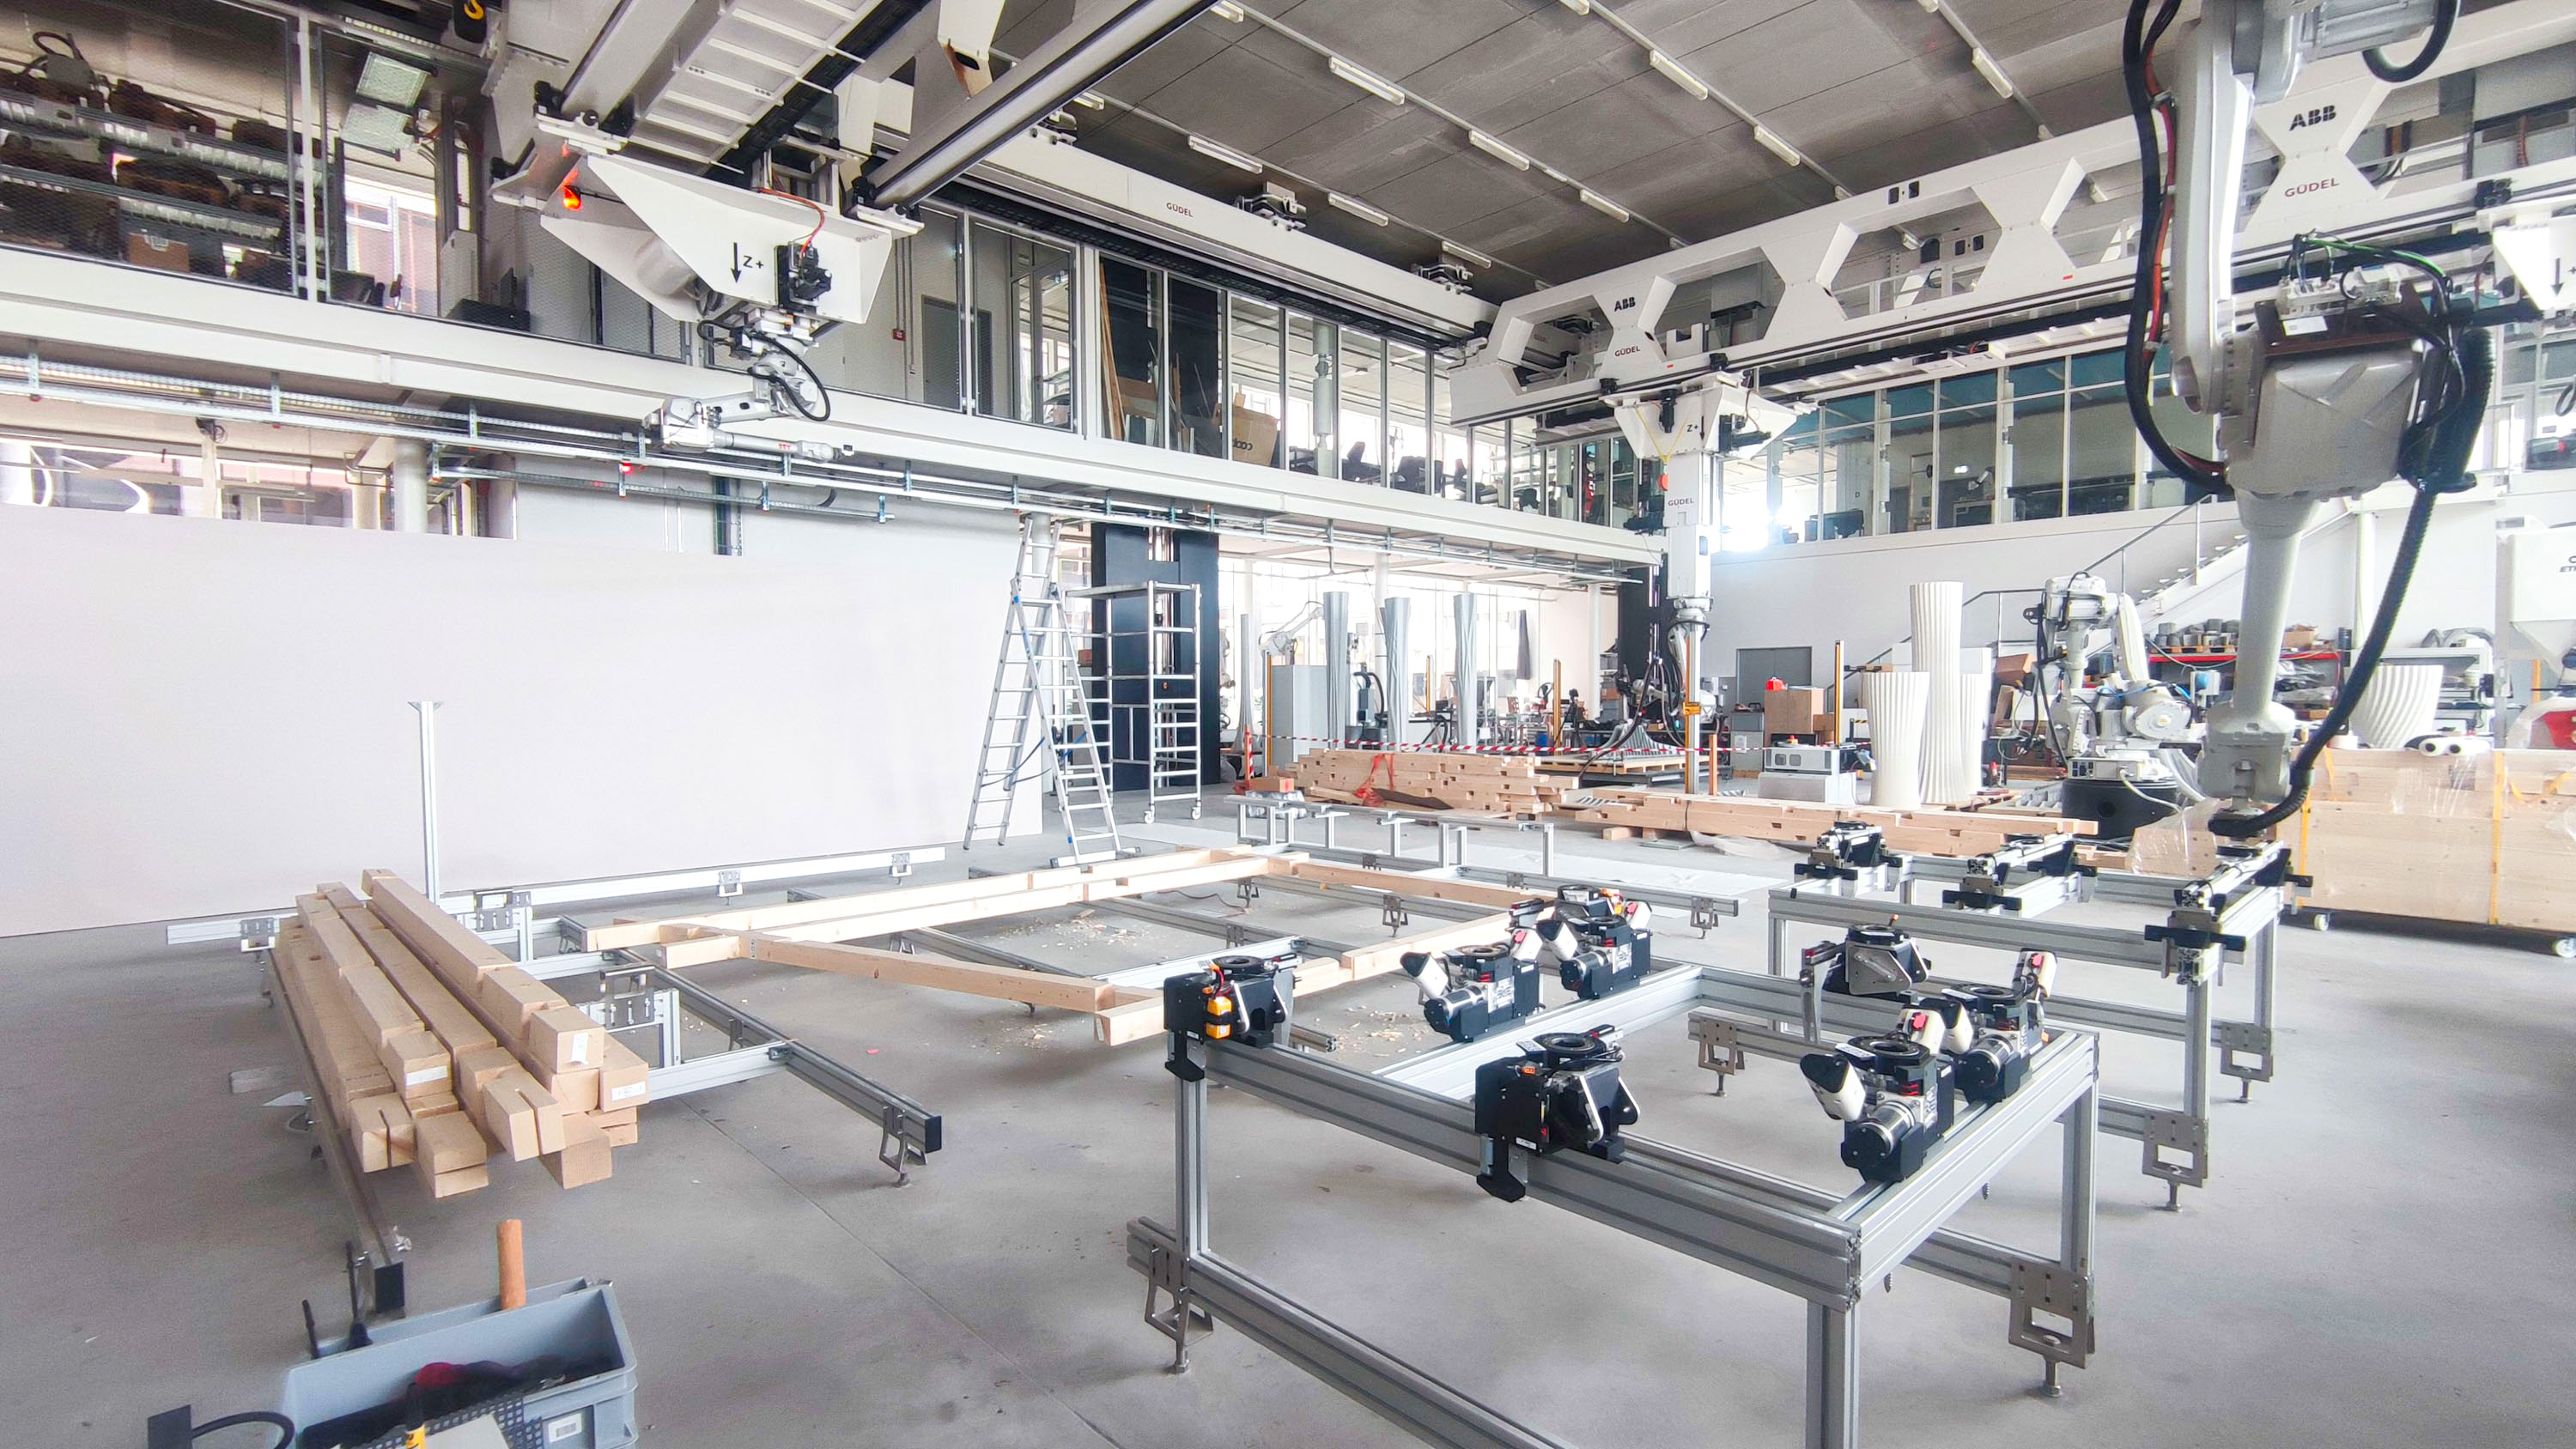
\includegraphics[width=0.99\textwidth]{images/10/Construction Area.jpg}
    \caption{Robotic construction area setup used for assembling CantiBox}
    \label{fig:robot-area-for-cantibox}
\end{figure}

\subsection{Designing new DiRT tools}
\label{subsection:discussion-designing-new-dirt-tools}

DiRT tools are modular in nature which allows them to fulfil different types of roles. For example, the role of the robotic clamps is to create a high compressive force locally at the area of the lap joints; The role of the screwdriver is similar but the assembly force is pulled from the middle of the joint and is also able to place a permanent fastener. While assembly tools are the only type of tools being developed in this thesis, it is possible to develop other types of DiRT tools based on the experience gained from this thesis. 

This section presents a systemic design approach for designing new DiRT tools. In order to demonstrate the design procedures and considerations, I will attempt to redesign the temporary scaffolding in CantiBox (see Figure \ref{fig:manual-scaffolding-cantibox}) such that it can be attached and detached automatically. I refer to this process of converting existing manual tools to a DiRT tool - DiRTify or DiRT-ification.

\begin{figure}[h!]
    \centering
    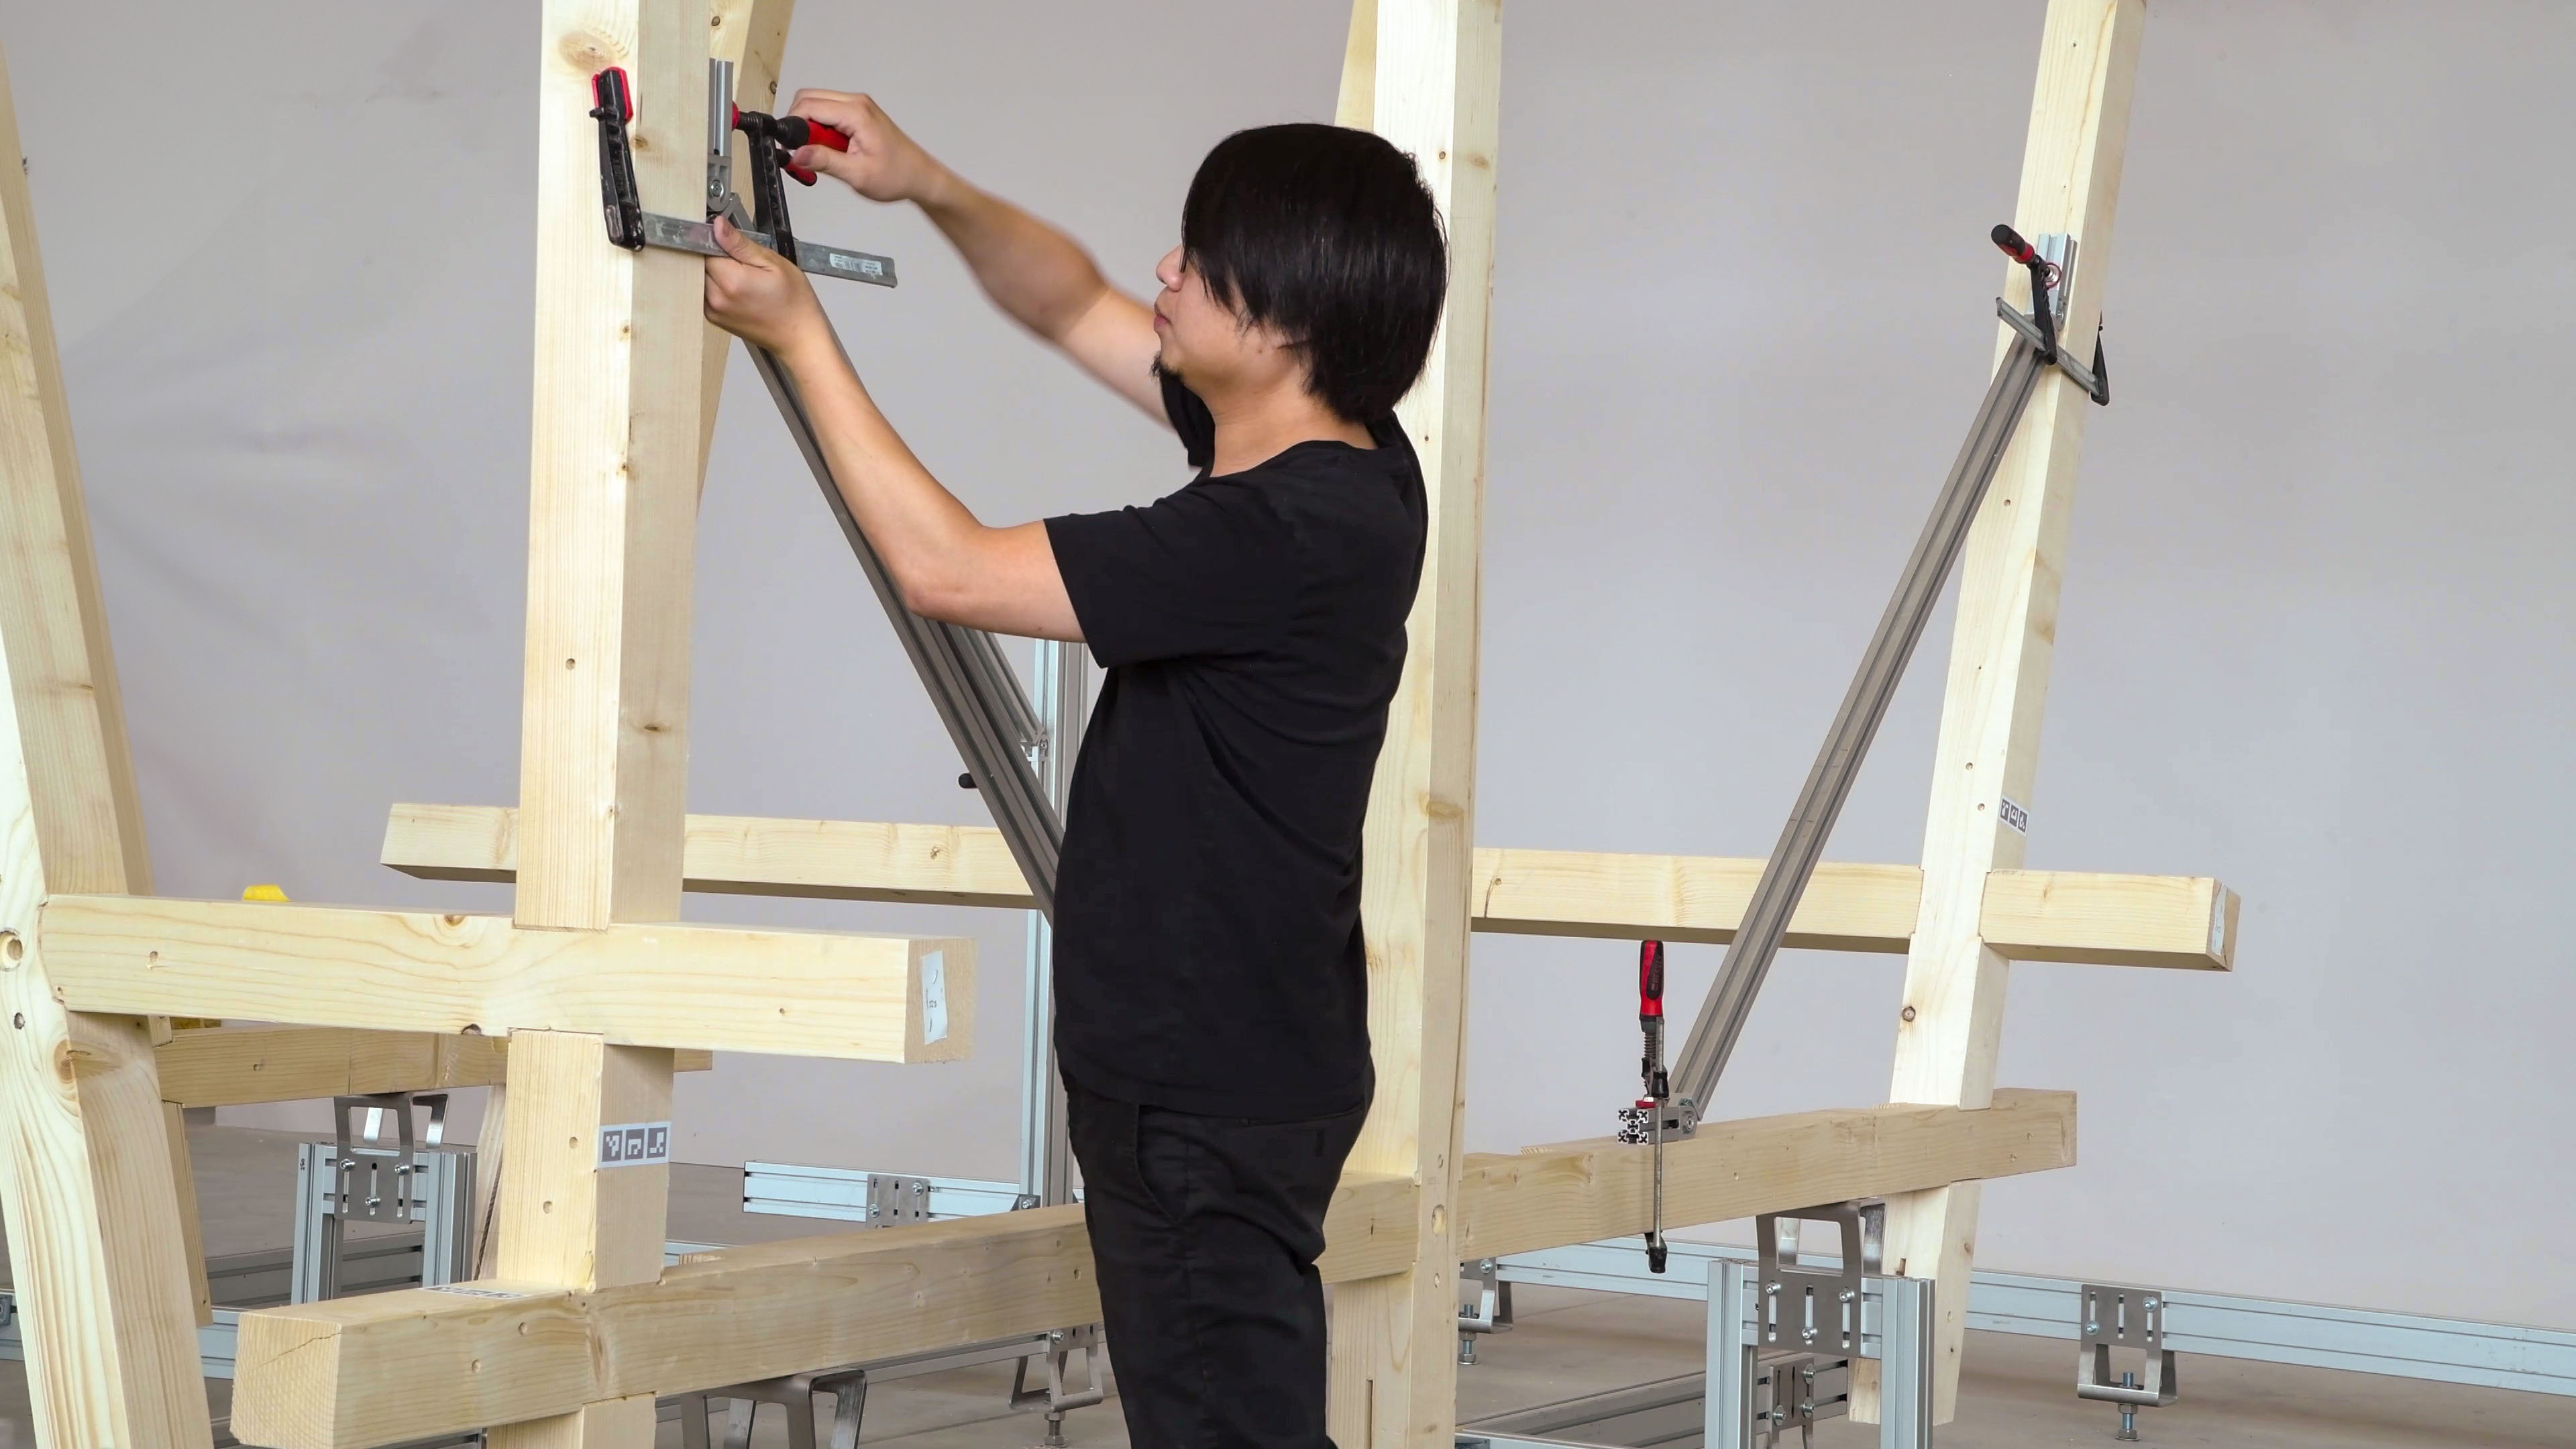
\includegraphics[trim=0mm 20mm 0mm 0mm, clip, width=0.99\textwidth]{images/10/Manual Attach Scaffolding.jpg}
    \caption{Manually attached scaffolding used during the construction of CantiBox}
    \label{fig:manual-scaffolding-cantibox}
\end{figure}

The design process starts by drafting the specifications of the tool, which corresponds to two main operational aspects - the task to be completed and how the tool is attached. Table \ref{table:example-specification-dirt-scaffolding} contains an example of the specifications drafted for the DiRT scaffolding:

\begin{table}[h!]
    \includegraphics[page=9, trim=25.4mm 130mm 25.4mm 33mm, clip, width=0.98\textwidth]{tables/Tables in Chapter 9 to 11.pdf}
    \caption{Example specifications for a DiRT scaffolding}
    \label{table:example-specification-dirt-scaffolding}
\end{table}

\FloatBarrier

When describing the task, it is necessary to analyse what kinematic actions are needed to perform the task, and if any essential parts are required. In this example, the scaffolding bar does not require any kinematic movement. However, in the screwdriver development, the screwdriver head and the pull screw were essential components.

When defining the geometrical flexibility of the task, be aware of its implications for the complexity of the tool. For example, if the scaffolding bar is to be extendable, an extra actuator is needed to do so. In general, it is best to avoid adding too much flexibility to the tool, as simplicity keeps the tool light and low cost. One potential opportunity for adjusting the dirt tool without adding an actuator is to use the robotic arm to adjust the tool. For example, the length of the scaffolding bar can be adjustable by a push or rotation delivered by the robotic arm before the bar is being picked up.

When designing the attachment method, it is best to first identify the direction of which the tools are attached and detached. Ensure the robot can reach into the area to perform the attachment and the detachment scenario is not blocked by the presence of newly assembled parts. Based on the assembly direction, the attachment mechanism can be detailed. This mechanism needs to ensure good registration accuracy with the workpiece, good stiffness after attachment and should be protected against accidental release. The pneumatic parallel gripper and electric pin gripper are good examples that can be reused. Because the tool is to be attached to the partially-assembled structure by the robot, alignment-correction method is likely necessary to achieve a high success rate. Based on the experience of this thesis, the camera-marker method proves to be quite robust. 

Based on the specifications, a design study can generate different design options. The following list provides a guideline for important metrics to evaluate when deciding which option to pursue:

\begin{description}
	\item [Choice of power source] Typically electric power is provided by an onboard battery. When the tool is attached to the robot, high-power electricity and pneumatic power can be provided through the docking adapter. Evaluate cost and power consumption per operation cycle.

	\item [Weight of the tool] Perform additional deviation analysis for typical attachment scenarios to make sure the tools can be hung from their intended locations without causing excessive deformation.

	\item [Implementation complexity and cost] Evaluate the choice of actuators and the required drivers and controllers. Typically, fewer actuators make the device simpler and lighter.

	\item [Chance of successful attachment] Based on the alignment mechanism and the choice of alignment correction mechanism, estimate the allowable tolerance and correction range. Evaluate the chance of successful alignment for typical attachment operations using the alignment-correction model. 

	\item [Risk of collision] Perform collision check for every key step during attachment, operation and detachment process. All collision objects should be considered, such as, robots, other tools, already-assembled structure, and ground foundation. If the tool is flexible to interact with geometrically different workpieces, perform multiple checks for each degree of freedom (at least one checks at each extreme of the flexibility and at the neutral position). Not all scenarios need to be collision free, for example, cases where multiple flexible dimensions are at their extremes can be exempted. The purpose of this evaluation is to get a sense of the design freedom. 

	\item [Command and control] Evaluate whether the standard wireless command control framework can be used. Evaluate if bandwidth and latency is sufficient, especially if camera feed is required.

\end{description}

Finally it is necessary to consider the placement of the docking adapter. The position of the adapter directly determines the position of the robot flange and the position of the robot wrist when the tool is attached. For spherical wrist robots, such as the one used in this thesis, the wrist can be approximated by a sphere. A special property of these robots is that the sphere’s position relative to the flange does not change with the movement of Joint 5 or Joint 6. Therefore, tool designers can use this sphere as a rule-of-thumb guidance to make sure there are no collisions with the parts being assembled.

In conclusion, the development of custom DiRT tools is a clearly defined mechatronics design process that is repeatable and adaptable to a wide array of applications. The systematic design approach presented here allows each new tool to be optimised for its specific task, while also maintaining compatibility with the overarching robotic system. By following these design guidelines and principles, engineers can create modular and versatile tools that extend the capabilities of the DiRT assembly system. 

\subsection{Robotic Platform}
\label{subsection:discussion-robotic-platform}

The robotic platform used for DiRT operations is generic in nature. The specific implementation can be adapted to on-site conditions and the target building size. This is similar to how cranes of different size, payload capacity and base condition (stationary vs mobile) are selected in the current construction practice. 

Table \ref{table:dirt-specifications} provides a list of robot specifications for DiRT operations that are crucial for achieving reasonable design freedom, efficiency, and safety during the construction process. It also includes how each specification can be determined according to the construction task in a generalised scenario. For timber frame construction, the values used for this thesis is included for reference, together with the recommended values concluded from the experience gained.

\begin{table}[hb!]
    \includegraphics[page=10, trim=25.4mm 60mm 23mm 33mm, clip, width=0.98\textwidth]{tables/Tables in Chapter 9 to 11.pdf}
    \caption{Crucial robot specifications for DiRT operations}
    \label{table:dirt-specifications}
\end{table}

The primary consideration in implementing the robotic platform is the kinematic arrangement. A popular approach, that is also used in this thesis, is the overhead gantry with an inverted robot arrangement. This arrangement offers overhead clearance to facilitate navigation in congested assembly areas. It is also the most common arrangement used in many of the integrated automated construction sites found in Japan \parencite{linnerAutomatedRoboticConstruction2013, potterJapanSkyscraperFactories2022}. Apart from its sturdiness, it provides other benefits such as attachment of vertical material transport robots and weather cover over the gantry.

There are alternative arrangements to the gantry-robot approach, one of which is crane-based robots, such as tower cranes or crawler cranes. They offer high lifting capabilities but face challenges controlling sway \parencite{neupertTrackingAntiswayControl2010} and rotation \parencite{liangRASRoboticAssembly2017}; Another alternative is robots based on articulating boom lifts, which provide good reachability but have lower payload capacities. These may be suitable for attaching and detaching DiRT tools but insufficient for lifting building components. 

In this thesis, the gantry-robot arrangement achieves a balance between accuracy, reachability and payload capacity suitable for timber frame assembly. However, for heavier construction components such as prefab-concrete and steel, it is likely that the role of heavy lifting and manipulating DiRT tools are distributed to two different robotic platforms, each optimised for their specific tasks.

In conclusion, the selection of an appropriate robotic platform for DiRT operations depends on the construction material and assembly process. While this thesis focused on the assembly of timber frame structures with integral timber joints, it is likely that actual on-site robotic platforms will need to accommodate a wider variety of components and processes. The specification of which will need to integrate and satisfy all requirements while maintaining flexibility.

\FloatBarrier

\subsection{Docking Adapter}
\label{subsection:discussion-docking-adapter}

In the previous sections, it was discussed that DiRT tools are modular and the robotic manipulator is generic. This leaves the interface between the two being the only unvarying aspect in a DiRT implementation. Much like the International Space Station's docking adapter, which unites and fosters cooperation among various space-faring nations, the DiRT docking adapter stands as a symbol of collaboration. It provides compatibility between new and old tools, those developed by different parties, and different robotic platforms deployed across diverse job sites.

The docking adapter is an automatic device that allows the robotic manipulator to pick up and attach a DiRT tool. A typical implementation consists of a pair of mechanical parts, one rigidly installed on the robot-side and the other one on the tool-side. An actuator within the mechanism performs locking or unlocking actions between the pair. The interface is often designed with tapered surfaces to correct for misalignments and to ensure docking repeatability. When docked and locked, the adapter serves as a strong and stiff mechanical connection between the arm and the DiRT tool and can provide electric and pneumatic power over the interface.

One of the most important specifications of the adapter is its payload capacity. Similar to the discussion in the previous chapter, the selection of a suitable capacity depends on how the entire DiRT system is integrated with other construction processes. Once this standard is set, all DiRT tool implementation is required to comply with its limitations. In this thesis, the docking adapter is implemented by adapting an existing off-the-shelf automatic tool changer \seeref{subsection:exploration-2-docking-adapter}. The specific model (SWA-040 by Schunk) was chosen because previous projects in the laboratory have donated them for reuse. Although it is slightly undersized for the timber beams, it was considered sufficient for demonstrating the DiRT system prototype. 

It is worth noting that the payload capacity of a docking adapter is directly related to its size. Therefore, overspecification of the adapter size does not only increase tool-side cost, but its physical size and weight can limit the performance of the tool. Therefore, in practice, it may be beneficial to have more than one adapter size. The largest of which is installed on the robotic platform and adapters between the adapters can be used to interface with smaller tools.

During the development of the automatic tool placement procedure, it was found that the docking tolerance of 2mm offered by the tool presented a challenge for robotic alignment. The solution was to add a camera on the robot side, target markers on the tool side, and develop an alignment algorithm to perform correction by moving the robot \seeref{subsection:exploration-4-camera-marker-hardware-on-docking-adapter}. While this method proves to be highly successful, an alternative solution would be to redesign the mechanical interface to allow for more tolerance. In addition to the pneumatic feedthrough, it would also be beneficial to include a power feedthrough for charging the on-board tool batteries while the tools are being handled \seeref{subsubsection:exploration-5-combined-operation-of-dirt-tools}. 

\FloatBarrier

\subsection{Wireless Communication System}
\label{subsection:discussion-wireless-communication-system}

In order to communicate wirelessly with the DiRT tools, it is essential to have a high-performance and robust radio communication system. While there are many matured wireless communication systems like Wi-Fi and ZigBee, they do not fully address the unique challenges and requirements of DiRT systems in a construction environment. For example, ensuring signal reliability in a construction environment with many occlusions is challenging but essential to the robot process. As many of the DiRT movements require synchronising movements with multiple tools and robots, any dropped connection will result in an emergency stop, causing a disruption to the process. Table \ref{table:dirt-wireless-specifications} lists the general requirements for a wireless communication system designed for DiRT operations:

\begin{table}[h!]
    \includegraphics[page=11, trim=25.4mm 70mm 25.4mm 33mm, clip, width=0.98\textwidth]{tables/Tables in Chapter 9 to 11.pdf}
    \caption{General requirements for a wireless communication system designed for DiRT operations}
    \label{table:dirt-wireless-specifications}
\end{table}


In this thesis, a custom network is implemented based on a low-cost sub-GHz radio transceiver (CC1101 by Texas Instruments) installed on each DiRT tool \seeref{subsection:exploration-2-radio-network}.The frequency and encoding is chosen to maximise signal reliability, and the radio is set to the maximum allowable power under licence-free operation. Although this was shown to be sufficient for operating the DiRT system in the lab, there are many shortcomings that should be improved in future implementation \seeref{subsection:exploration-5-wireless-radio-latency}.

Note that the wireless communication system is the software and electronics counterpart of the docking adapter. Once a standard is chosen, subsequent DiRT development is constrained by the choice. Therefore, careful consideration and physical tests are necessary to ensure that the requirements listed above are met. In conclusion, a custom wireless communication solution is needed for DiRT operations to ensure its performance and reliability.

\subsection{Control Systems}
\label{subsection:discussion-control-systems}

In order to coordinate all the robotic hardware to perform a series of planned tasks, a complex control system is needed. In order to follow a modular development process, a distributed control system (DCS) model is adopted. Specifically, the control, monitor and synchronising tasks are separated into a layered stack of software that communicates with each other \seeref{subsection:exploration-2-distributed-control-system}. Figure \ref{fig:communication-software-relationship} shows the relationship between all the control software used in this thesis, arranged according to a DCS model. The communication channel is labelled on the arrows. In addition, a set of command-response protocols were also developed for two way communication between each layer. 

\begin{figure}[ht!]
    \centering
    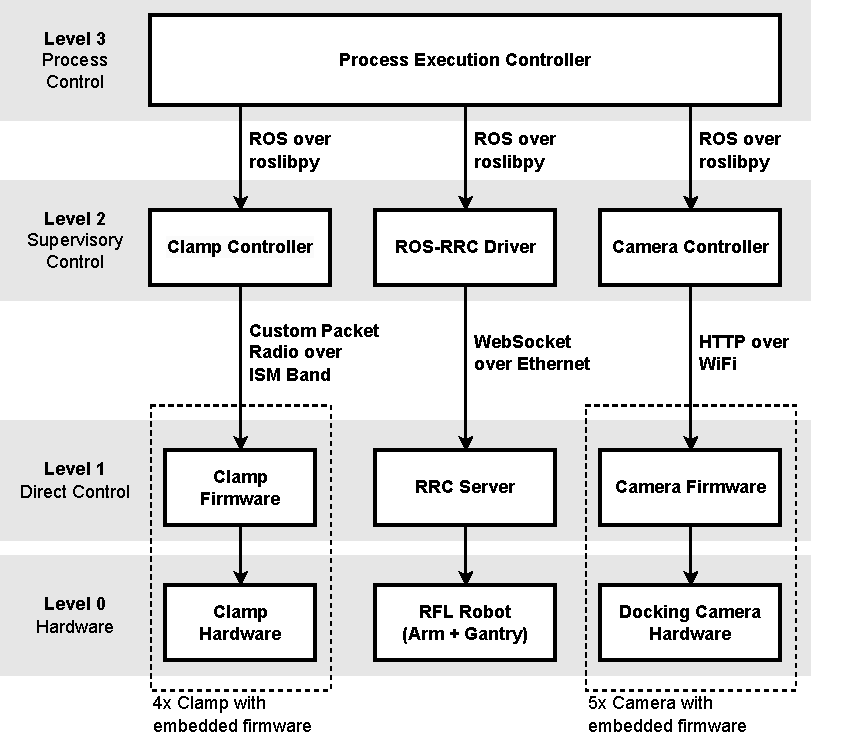
\includegraphics[width=0.99\textwidth]{images/10/Control Software Relationships.pdf}
    \caption{Communication relationship between control software components used in this thesis}
    \label{fig:communication-software-relationship}
\end{figure}

This software arrangement with an overarching process execution controller is generic for any multi-controller scenarios. Level 1 or Level 2 controllers can be added if additional hardware is needed for the process. In this case, the Level 3 Process Execution Controller only needs to be revised to manage the new connection and to support the new commands \seeref{subsection:exploration-3-standalone-process-execution-controller}. 

Experience has shown that the use of compas\_rrc \parencite{fleischmannCOMPASRRCOnline2020} to send commands between Levels 2 and 3 is extremely flexible. Specifically, the `Instructions` class can be used to encapsulate newly developed instruction sets, such as requesting a status report, setting states, or starting an action. It also supports synchronous and asynchronous command modes, which is essential for managing long-running motion tasks. In addition, the use of ROS messaging system by compas\_fab allows easy addition of Level 2 controllers, even if they are running on a different computer. 

\FloatBarrier
\section{Conclusion of Discussion}
\label{section:conclusion-of-discussion}

In conclusion, this chapter has offered new insights into the automatic timber frame assembly problem and highlighted the discoveries that are relevant beyond the initial scope. Throughout the chapter, several areas have been identified where the DiRT timber assembly system could be improved to increase reliability, flexibility and efficiency. The discussion also covered how the DiRT concept could be implemented on future construction sites and generalised for other construction systems. 

In some parts, the research has reached limits of what can be done within the scope of the assembly process and further progress has to be made together with upstream and downstream construction partners. This chapter has also raised many new challenges, questions and unexplored knowledge gaps that require the involvement of various domain experts. Future research should concentrate on fostering interdisciplinary collaborations to develop innovative solutions for these challenges.

% \chapter{New Hypothesis - Probabilistic Model of Spatial Alignment Success}
\label{chapter:new-hypothesis}
\chaptermark{New Hypothesis}

In this chapter, we will explore the concept of ``\textbf{Successful Alignment}" as a sub-problem of "Successful Assembly" and model it with a probabilistic approach. After observing the construction of the three demonstration structures, assembly success is dependent on two main factors: good alignment and high assembly force. While assembly force is specific to the assembly of integral timber joints, alignment is a generic challenge that affects all assembly processes, particularly those involving spatial assembly.

A robotic assembly process can be seen as a continuous chain of automatic operations. Within this chain, there are certain critical moments where good alignment accuracy is crucial before the process can continue successfully. By seeing every one of these moments as a challenge, where there is a certain probability of success, we can understand the overall ``Successful Assembly" as a combination of discrete probabilistic events.

\textbf{Alignment accuracy}, being a prerequisite for successful assembly, was a core challenge throughout this thesis, appearing in various forms and addressed at multiple stages of development. The initial focus was on aligning timber joints with each other to ensure proper closure, leading to the development of chamfered joint edges and high-force robotic clamps for passive guidance \seeref{subsection:exploration-2-clamping-joints-with-chamfered-edges}. As the research progressed towards automatic DiRT tool placement, additional alignment scenarios were required to attach and detach tools automatically, presenting unique challenges and necessitating the development of active correction methods \seeref{subsection:exploration-4-camera-marker-alignment-correction-system}.

Reflecting on the three demonstrator construction, it became apparent that alignment and corrections were not always successful, as deviations could be larger than expected. This prompted an investigation into the sources of these deviations and the potential for developing models to better predict them. Towards the end of this thesis, after examining all alignment scenarios, a pattern for modelling the alignment and correction problem emerged. This led to a new hypothesis—a statistical model capable of predicting the probability of successful alignment by considering deviation, tolerance, and the correction method applied.

In this chapter, I will introduce the new hypothesis centred around the probabilistic model of spatial alignment success and explore its implications for the broader assembly domain. It is important to note that this model has not been tested within the scope of this thesis but the current findings shows that the model is in agreement with the observations. Further studies are required to confirm its completeness, validity, and practicality. 

\section{Modelling Alignment and Correction}
\label{section:new-hypo-modelling-alignment-correction}

Let's begin by looking at the Table \ref{table:alignment-scenarios}that outlines all the alignment scenarios performed. Since we are using one robot for the assembly, the scenarios can all be described as ``Some part(s) on the robot-side attempting to align with some other part(s) on the stationary-side". 

\begin{table}
    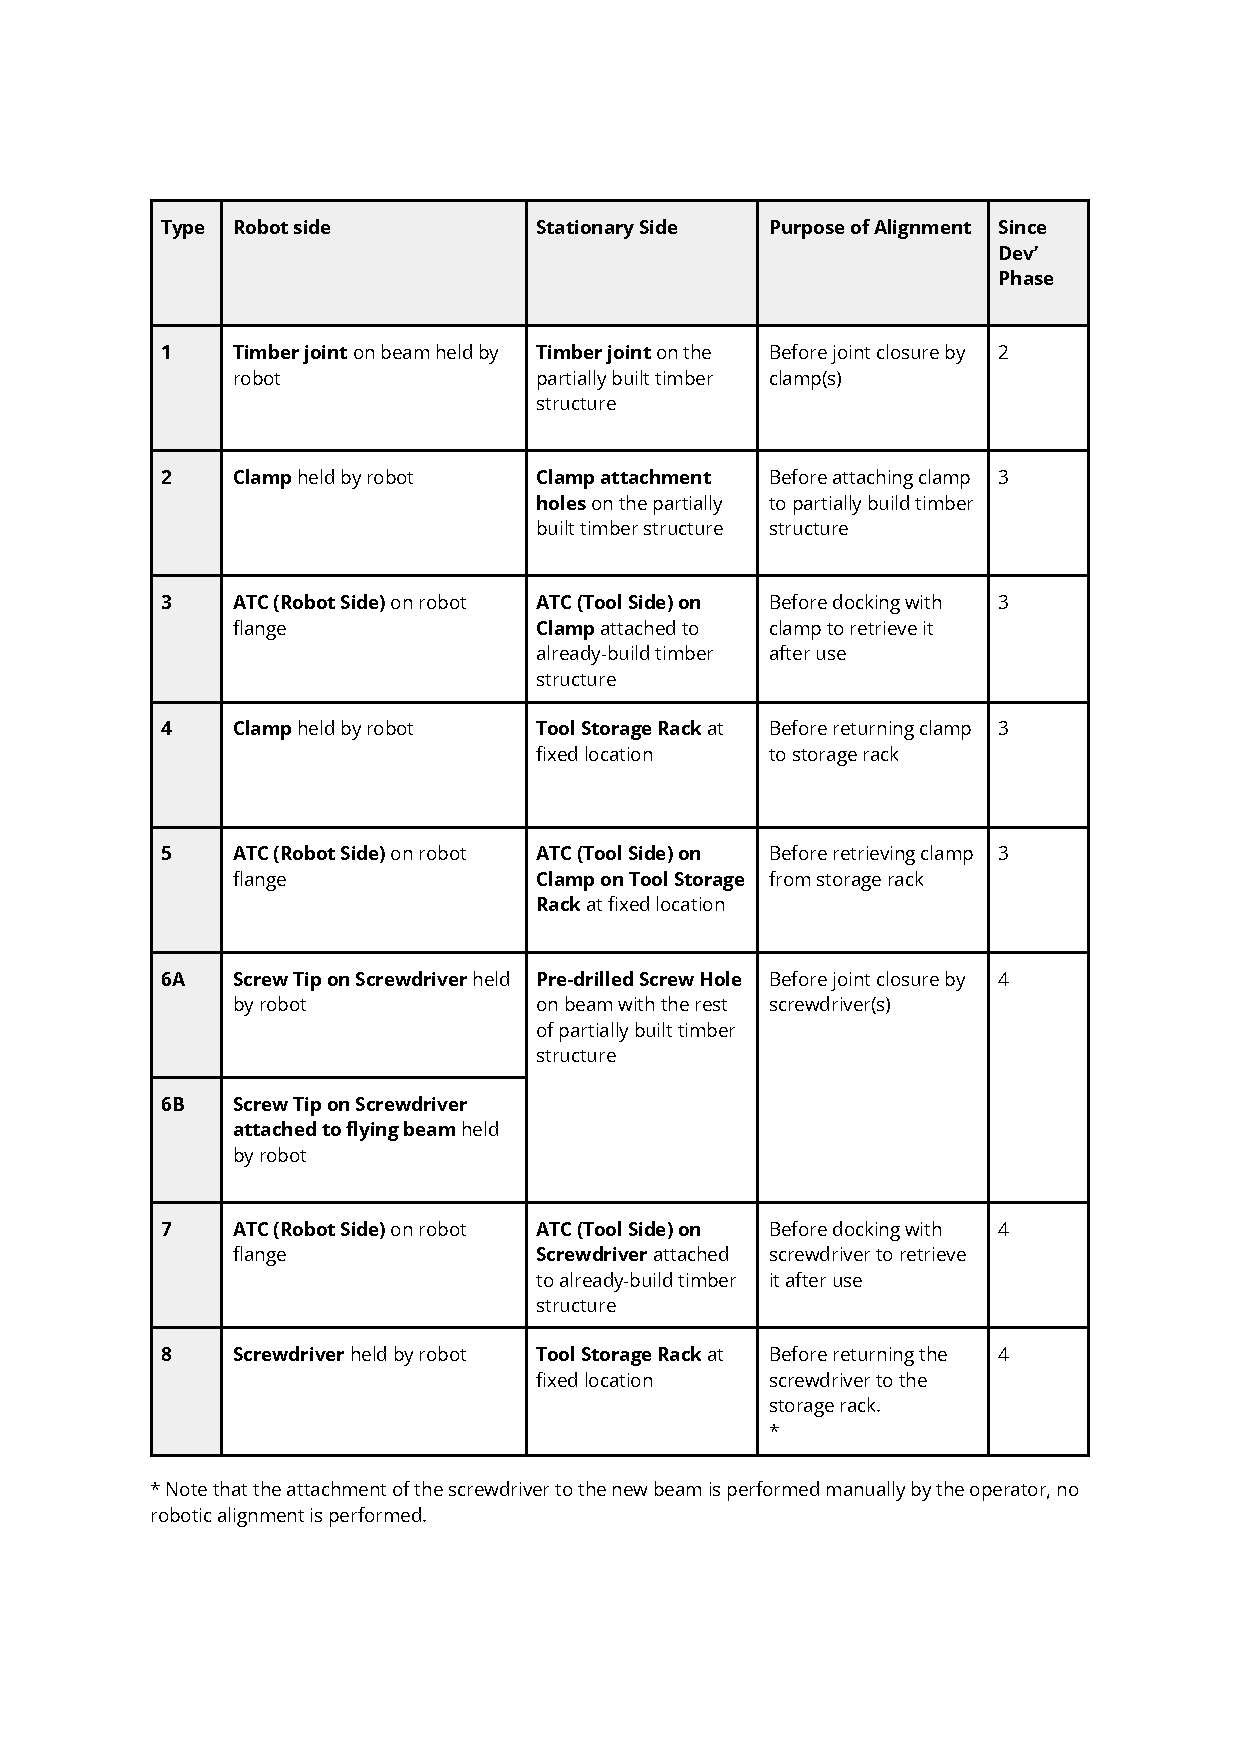
\includegraphics[page=1, trim=25.4mm 35mm 25.4mm 33mm, clip, width=\textwidth]{tables/Tables in Chapter 9 to 11.pdf}
    \caption{Alignment scenarios performed in the demonstrations}
    \label{table:alignment-scenarios}
\end{table}

\subsection{Alignment-Correction Model}
\label{subsection:new-hypo-alignment-correction-model}

Observations of the three demonstrations (from Development Phase 3 to 5) indicated that there are many different factors affecting the amount of deviation in each of the alignment scenarios. They affect whether the total pairwise deviation can be corrected and thus the chance of successful assembly. Below are some examples of the success factors:

\begin{description}[style=unboxed] % Environment provided enumitem package
	\item [Tight tolerance, deviation of partially assembled structure] When picking up tools from the structure (types \#3 and \#7), the alignment between robot-side ATC and tool-side ATC has a very low chance of success \seeref{subsection:exploration-3-docking-adapter-misalignment}. This may be caused by a combination of the small allowable tolerance (2mm) governed by the design of the ATC and the high deformation of the partially built structure from which the tool is hanging. 

	\item [Correction range] Comparing the two joint closure methods, screwing closure (type \#6) have a much higher success rate than clamping closure (type \#1). This may be explained by the pointy tip of the screwdriver aiming at a relatively large pre-drilled hole.

	\item [Deviation] When retrieving tools from and returning tools to the stationary tool storage (type \#4, \#5 and \#8), the alignment has a very high success rate when compared to other alignment types. This may be explained by the fact that tool storage alignment is performed manually by teaching, there is no deviation of the tool storage afterwards and the robotic platform is repeatable. In other alignment scenarios, the target is novel and may be deformed from its designated location.

	\item [Payload] During the transport of a beam to the work area, if the beam is very heavy \seeref{subsection:exploration-4-heavy-beam-caused-robot-overload}, or if the grasp is not near the middle, the chance of success is low. 

\end{description}
In order to create a unified model to include different deviation factors, I first draw inspiration from the study of error in machine design, which uses the concept of structural loop to identify sources of error.

% 1 Image  
\begin{figure}
    \centering
    \includegraphics[width=0.99\textwidth]{example-image-a}
    \caption{Figure Caption}
    %\label{fig:unique-figure-label}
\end{figure}

The diagram above shows a Type 1 alignment scenario where two joints needs to be aligned. We can identify two \textbf{structural chain }that stems from a fixed reference (ground or ceiling) towards the two points of alignment \parencite{slocumPrecisionMachineDesign1992}. On the robot-side, the timber joint is located on a beam held by the robot through a gripper. On the stationary-side, the timber joint is located on the partially built timber structure, which is located on a temporary platform. In a perfect scenario, the alignment point (or pose) on each side should both be equal to the target that is extracted from the CAD model. I refer to this as the ‘\textbf{ground truth}’. In reality, due to imperfection of each component in the structural loop, both alignment points will be deviated from the ground truth. These imperfections include stiffness of the timber material, accuracy of the prefabricated timber parts, deformation of the machine parts and inaccuracy of the robotic control systems. 

The second inspiration is taken from the study of reliability in the field of systems engineering, for the use of probability to model success and failure \parencite{hallmannToleranceAllocationTolerancecost2020}. Consider the deviation between the two alignment points, we can assume it behaves like a random variable. This allows us to model it as a continuous probability distribution that can be analysed using statistical methods. Specifically, using the cumulative distribution function\footnote{ In probability theory and statistics, the cumulative distribution function (CDF) of a real-valued random variable X, evaluated at x, is the probability that X will take a value less than or equal to x. } (CDF) to analyse the worst-case deviation.

The two graphs below can help us understand CDF in a graphical way. Let us consider the deviations between the two alignment points. Assuming it is a continuous random variable, its distribution can be graphed using the probability density function, where the X axis is the deviation and Y axis is the probability density. The area under the graph represents all possible values, and therefore it has an area of 1. If we want to find the probability that the actual deviation is less than a certain threshold, we can draw a vertical line at that threshold and find the area on the left-hand side. Mathematically, this can be represented by $F_D (x) = P (D \leq x)$, where $F_D ()$ is the CDF of deviation $D$, $P$ is the probability density function (PDF), and the $T$ is the threshold to be analysed.

In practice, it is possible to quantify the PDF of a random variable by measurement, model fitting and simulation. Details of which will be presented later in the section.

% 1 Image  
\begin{figure}
    \centering
    \includegraphics[width=0.99\textwidth]{example-image-a}
    \caption{Figure Caption}
    %\label{fig:unique-figure-label}
\end{figure}

The use of PDF and CDF is related to, but different from the typical accuracy representation in the field of robotics. When discussing machine accuracy, it is more common to measure trueness (difference between ground truth and statistical mean) and precision (standard deviation of the distribution). 

However, for the purpose of assembly, we are interested in the \textbf{worst-case deviation }between the two alignment points for determining whether the alignment is sufficiently good. The use of CDF allows us to directly model the alignment problem by relating the threshold value and the probability of the actual value falling within range. 

Given the following variables: 

\begin{itemize}[nosep]
	\item $d$ is the measured deviation of the two alignment points across the open structural loop. It is assumed to be a random variable because of the random imperfections in the system. 

	\item $D$ is the probability distribution of the random deviation $d$, 

	\item $x$ is a variable representing a deviation threshold to be analysed 

	\item $K_D \in (0,1)$ represents the probability that $d$ takes on a value less than or equal to $x$. 

\end{itemize}

Using the cumulative distribution function $F_D ()$ we can define a variable $K_D \in (0,1)$ to be the probability that $d$ takes on a value less than or equal to $x$: 

\begin{equation}
    K_D = F_D (x)
\end{equation}

In addition, we model the \textbf{allowable assembly tolerance} of the mating features, such as the gap in a pin-in-hole assembly or the gap on a loose joint pair. From the perspective of the mating features, it is the maximum threshold of deviation d such that assembly is still successful. We can define it using: 

\begin{itemize}
	\item $T$ as the allowable assembly tolerance 
\end{itemize}

If a \textbf{correction mechanism} is used, such as chamfered edges passive correction or camera-marker active correction. We can model the properties of the correction mechanism or process using: 

\begin{itemize}[nosep]
	\item $C_{Range}$ as the maximum correctable range (e.g. size of chamfered joint edge)

	\item  $K_D \in (0,1)$ as the success rate of the correction method. 

\end{itemize}

\textbf{The numerical representation and units }have to be consistent for $d$, $x$, $T$, $C_{Range}$ and $C_{Residual}$. For the sake of simple arithmetics, the subsequent explanation will only consider the absolute Cartesian distance for the deviation. Therefore it is represented as a signless real number. Alternatively, a transformation consisting of translation and rotation can be used. However, the transformation arithmetics will be outside the scope of this explanation. 

Finally, the probability of successful assembly is represented by $S \in (0, 1)$. Using the defined variables, I propose the following Alignment-Correction Model to relate S as a function of d with three intervals: 

\begin{description}[style=unboxed] % Environment provided enumitem package
	\item [No correction needed] if $d \le q$ T then $S = 1$\\ (Explanation: No correction is needed because the deviation is within the allowable tolerance.)

	\item [Correction success] if $T < d \leq C_{Range}$ \\ (Explanation: The deviation is within the range of the correction mechanism and its residual deviation is within the allowable tolerance.)

	\item [Correction failure] if $C_{Range} < d$ then $S = 0$

\end{description}
The function can be expressed by: 

\begin{subequations} \label{eq:probability-of-success}
  \begin{empheq}[left={S(d) = }\empheqlbrace]{align}
     1 &\text{ , if } x \le 0 \label{eq:probability-of-success-I}\\
     K_c &\text{ , if } T < d \le C_{Range} \label{eq:probability-of-success-II}\\
     0 &\text{ , if } C_{Range} < D \label{eq:probability-of-success-III}
  \end{empheq}
\end{subequations}

Note that some correction mechanisms do not correct the deviation to zero but to within a certain range. It is important for this residual deviation after correction to be smaller than $T$, such that it can be accommodated by the allowable tolerance. In practice, the allowable tolerance and residual deviation are physical properties of the mating feature and the correction system, which can always be satisfied by proper design of the correction mechanism. For example, in the camera-marker correction system, the convergence value is designed to ensure successful alignment with the docking adapter.

Using the CDF of $D$ in Equation \ref{eq:probability-of-success} , the probability of $d$ landing inside interval $I$ is 

\begin{equation} \label{eq:probability-interval-I}
    K_I = F_D (T)
\end{equation}

For landing in interval $II$, 

\begin{equation} \label{eq:probability-interval-II}
    K_{II} = F_D (C_{Range}) - F_D (T)
\end{equation}

The following diagram graphically represents the distribution of alignment points around the ground truth graphically. The two circles define the boundary between interval I and II and III. The radius of the inner circle is equal to the upper bound of interval I where $d = T$, the radius of the outer circle is the upper bound of interval II where $d = C_{Range}$. 

The graph on the right depicts the same concept, but plots the probability of successful assembly $S(d)$ with respect to $d$ and the labels are the probability of their occurrence from Equations \ref{eq:probability-interval-I} and \ref{eq:probability-interval-II}.

% 2 Horizontal Image  
\begin{figure}
    \centering
    \begin{subfigure}[b]{0.49\textwidth}
        \centering
        \includegraphics[width=\textwidth]{example-image-a}
        \caption{Sub figure caption}
        %\label{fig:unique-subfigure-label}
    \end{subfigure}
    \hfill
    \begin{subfigure}[b]{0.49\textwidth}
        \centering
        \includegraphics[width=\textwidth]{example-image-b}
        \caption{Sub figure caption}
        %\label{fig:unique-subfigure-label}
    \end{subfigure}
    \caption{Figure Caption}
    %\label{fig:unique-figure-label}
\end{figure}

We can find the combined probability of success $S$ for all three zones. Note that interval $III$ is ignored because the probability of success is zero. Using the summation of probability:

\begin{equation} \label{eq:probability-of-three-intervals}
    S = K_I \cdot S_I + K_{II} \cdot S_{II}   
\end{equation}

Expending the terms using Equations \ref{eq:probability-of-success}, \ref{eq:probability-interval-I} and \ref{eq:probability-interval-II}:

\begin{equation} \label{eq:probability-expanded}
    S = F_D(T) \cdot 1 + (F_D (C_{Range}) - F_D(T)) \cdot K_C
\end{equation}

After arranging some terms:

\begin{align} \label{eq:probability-expanded-rearranged}
    S &= F_D(T) + F_D (C_{Range}) \cdot K_C - F_D(T) \cdot K_C \nonumber \\
      &= F_D(T) \cdot (1 - K_C) + F_D(C_{Range}) \cdot K_C 
\end{align}

In this thesis, in the cases where tight fitting joints are aligned with each other, there is zero tolerance $(T = 0)$ , thus $F_D(T) = 0$. In this special case, the formula can be simplified to:

\begin{equation} \label{eq:probability-when-zero-tolerance}
    S = F_D(C_{Range}) \cdot K_C 
\end{equation}

\subsection{Application}
\label{subsection:new-hypo-model-application}

There are many ways that the model can be used. For example, to design a robotic system for a given structure with a \textbf{predictable success probability}, it is possible to check all the alignment scenarios (after TAMP is performed with the given robots, tool setup and design) within the process to determine its success probability. 

Given $N$ steps in a process, and each step has a success probability of $S(i)$ where $i$ is the index of a step. If success at each step is required for an overall success, the total probability of success $S$ can be found by multiplying the success probabilities of each step together.

\begin{align} \label{eq:total-probability-success}
    S &= S(1) \times S(2) \times \cdots \times S(N)\nonumber \\
      &= \prod_{i=1}^{N} S(i)
\end{align}

If we want to determine the average percentage of steps that are likely to succeed, we can do so by finding the average success probability $A$ across all steps. This can indicate how frequently an operator has to attend to an anomaly.

\begin{align} \label{eq:average-step-success-probability}
    A &= (S(1) + S(2) + \ldots + S(N)) \times \frac{1}{N}\nonumber \\
      &= \left(\sum_{i=1}^{N} S(i)\right) \times \frac{1}{N}
\end{align}

Note that the distribution of $D$ is dependent on the states of the robot and parts, and the value of $T$ depends on the alignment scenario. Therefore the value of $S$ is unique for each alignment in the entire process. It is easy for a computer to check all the alignment moments and visualise those with low success probability. This can help the production engineer identify problematic situations and take corrective actions. For example, to reduce the deformation of a partially-assembled structure by adding scaffolding, changing its assembly sequence or introducing diagonal bracing elements.

Another application is for designing the assembly details. We can identify if there is a systemically low success rate for a certain type of alignment. This may indicate that the tolerance or the correction mechanism for that type of scenario has to be adjusted. For example, by increasing the size of the edge chamfer or the field of view of the camera system. It is even possible to automatically assign the appropriate amount of edge chamfer to each joint until a satisfactory success rate is achieved.

It is also possible to use the model as a comparison tool when choosing robotic system components. For example, we can compare the implication of choosing a specific robotic arm, gantry, or docking adapter. 

In conclusion, the Alignment-Correction Model allows us to analyse and predict the success rate of various assembly alignment scenarios in a robotic process. By taking into account deviation, tolerance and the correction method, this model enables production engineers, system designers and structure designers to identify potential problems, make informed decisions and predict execution outcomes. It is generalisable, mathematically simple and can be implemented computationally to allow quick and comprehensive check of all the alignment scenarios. These factors are important to ensure an efficient fabrication-aware design process.

\subsection{Chaining Deviation}
\label{subsection:new-hypo-model-chaining-deviation}

In the previous section, we have assumed the deviation to be a probability distribution. In this section, we talk about the procedures to quantify this distribution. 

Refer to the structural loop diagram. We can see that each side of the open loop consist of a number of components between the fixed ground and the alignment point. Assuming each of these components are affected by random imperfections, each of them contribute to the deviation, and accumulate at the point of alignment. The total deformation on each link can therefore be modelled as a forward kinematics problem where the deviation caused by each component is modelled as a rigid transformation $[Z]$ and the geometrical distance for each link is modelled as rigid transformation $[X]$. For a given chain $P$ The general kinematic chain equation allows the total chain deviation $T_P$ to be computed:

\begin{equation} \label{eq:one-chain-deviation}
    [T_P] = [Z_{P1}][X_{P1}][Z_{P2}][X_{P2}] \cdots [X_{P_{n-1}}][Z_{Pn}] 
\end{equation}

Where total deviation $d$ between the two alignment points on chain $P$ and $Q$ can be found by:

\begin{equation} \label{eq:two-chain-deviation}
    d = [T_P][T_Q]^T 
\end{equation}

While this representation of $d$ using rigid transformation is quite accurate, the complex representation is hard to be used for statistical analysis. To simplify the analysis, we can consider only the absolute positional deviation in each of these components, which can be represented by a single number. In practice, the rotation component is often small enough and the Abby error associated with it is small. For a conservative analysis, the worst-case combined deviation of $N$ links in the structural chain $P$ can therefore be computed by:

\begin{equation}
    d_P = d_{P1} + d_{P2} + \cdots + d_{PN}
\end{equation}

And the total deviation $d$ between the two alignment points on chain $P$ and $Q$ can be found by:

\begin{align} \label{eq:deviation-with-two-links}
    d &= d_P + d_Q \nonumber\\
      &= d_{P1} + d_{P2} + \cdots + d_{PN} + d_{Q1} + d_{Q2} + \cdots + dQN 
\end{align}

Because of the simple summation, there is no more differentiation between the elements in either one of the chains. All the links can be treated in the same way. Therefore, for a structural loop with N links in total, d can be decomposed into:

\begin{equation} \label{eq:deviation-with-all-links}
    d = d_1 + d_2 + \cdots + d_N
\end{equation}

Recall that each of the deviation components is a random statistical distribution, and they are independent of each other. We can expand the CDF of the total $d$ into its constituting components. We can make use of the Joint Cumulative Distribution Function identity:

\begin{equation}
    F_{XY}(x,y) = F_X(x) \cdot F_Y(y)
\end{equation}

For a structural loop with $N$ links on both chains, the $F_D(d)$ evaluated at $d$ can be expanded. 
\begin{equation}  \label{eq:probability-with-all-links}
    F_D(d) = F_1(d_1) \cdot F_2(d_2) \cdot \cdots \cdot F_N(d_N)
\end{equation}

Where $F_i(d_i)$ is the CDF of the link $i$ evaluated at $d_i$. Each of these distribution functions can be created from statistical measurements or by probabilistic simulation. Details of which will be presented later.

Finally, this function can be used in Equations \ref{eq:probability-expanded-rearranged} and \ref{eq:probability-when-zero-tolerance} of the model. The relationship of $d$ and $d-1, d-2, \cdots , d-N$ is described in equation \ref{eq:deviation-with-all-links}. During computation, an optimization function can be used to find the values of $d-1, d-2, \cdots , d-N$ such that it will maximise the probability of success in Equations \ref{eq:probability-expanded-rearranged} and \ref{eq:probability-when-zero-tolerance}.

In conclusion, the simplification of the deviation from transformation to measuring only absolute distance, makes the computation of accumulated deviation much simpler. There are two major sources of inaccuracy. The first is an underestimation of error, because Abby error resulting from the chained rotational deviation is not considered. The second is an overestimation of error due to the summation of absolute distance compared to the transformation-based analysis using Equations \ref{eq:one-chain-deviation} and \ref{eq:two-chain-deviation}.

% 1 Image  
\begin{figure}
    \centering
    \includegraphics[width=0.99\textwidth]{example-image-a}
    \caption{Figure Caption}
    %\label{fig:unique-figure-label}
\end{figure}

Depending on the nature of the deviation in the link, there are different methods of obtaining its statistical distribution. All of them require fitting a probability distribution to a series of measured data or properties. Different distributions can be selected depending on the shape of the measured data as long as an effective CDF can be applied to the distribution. Below are some examples of simple deviations and how they can found:

\begin{table}
    \includegraphics[page=2, trim=25.4mm 130mm 25.4mm 33mm, clip, width=\textwidth]{tables/Tables in Chapter 9 to 11.pdf}
    \caption{Examples of deviations}
    % \label{table:}
\end{table}

\FloatBarrier

% 1 Image  
\begin{figure}
    \centering
    \includegraphics[width=0.99\textwidth]{example-image-a}
    \caption{Figure Caption}
    %\label{fig:unique-figure-label}
\end{figure}

Consider an example shown in Figure \ref{fig:?} depicting a type \#1 joint-to-joint alignment scenario. For simplicity sake, the beam being assembled contains nly one mating joint. The photo depicts the connectivity chain on the robot side P and stationary side Q at the alignment moment. The possible source of deviation and their quantification method for all parts and interfaces are listed in Table \ref{table:deviation-robot-side} and \ref{table:deviation-stationary-side}. The estimated deviation $d$ and the probability $F(d)$ in the experiment setup is listed for the purpose of an example, they are not derived from actual measurement.


\begin{table}
    \includegraphics[page=3, trim=25.4mm 30mm 25.4mm 33mm, clip, width=\textwidth]{tables/Tables in Chapter 9 to 11.pdf}
    \caption{Possible deviation and their quantification method on Robot-Side}
    \label{table:deviation-robot-side}
\end{table}

\begin{table}
    \includegraphics[page=4, trim=25.4mm 165mm 25.4mm 33mm, clip, width=\textwidth]{tables/Tables in Chapter 9 to 11.pdf}
    \caption{Possible deviation and their quantification method on Stationary-Side}
    \label{table:deviation-stationary-side}
\end{table}

\textbf{The total deviation} $d$ (mm) between the two alignment points can be computed using Equation \ref{eq:deviation-with-two-links}:

\begin{align}
    d &= d_P + d_Q \nonumber\\
      &= (0.5 + 5 + 0.5 + 0.5 + 0.5 + 1 + 0.5 + 1) + (0.5 + 2 + 2 + 2)\nonumber\\
      &= 9.5 + 6.5\nonumber\\
      &= 16\nonumber
\end{align}

The probability of the deviation $F_D(d)$, when $d = 16$ can be computed using Equation \ref{eq:probability-with-all-links}:

\begin{align}
    F_D(d) &= F_x(x) \cdot F_Y(y) \nonumber\\
      &= (1 \cdot 0.95 \cdot 1 \cdot 1 \cdot 1 \cdot 1 \cdot 0.95 \cdot 0.95) \cdot (1 \cdot 1 \cdot 1 \cdot 0.95)\nonumber\\
      &= 0.857375 \cdot 0.95\nonumber\\
      &= 0.814506\nonumber
\end{align}
The result of this calculation can also be understood as $F_D(16) = 0.814506$ because $d = 16$.

Consider that there is no tolerance in this tight joint, tolerance $T$ is 0 mm. Assuming that the correction range of the edge chamfer $C_{Range}$ is 16 mm, and that it has a $K_C$ of $0.95$. We can apply Equation \ref{eq:probability-when-zero-tolerance} to determine the probability of successful assembly $S$:

\begin{align}
    S &= F_D(C_{Range}) \cdot K_C \nonumber\\
      &= F_D(16) \cdot 0.95 \nonumber\\
      &=  0.814506 \cdot 0.95 \nonumber\\
      &= 0.77378 \nonumber\\
\end{align}

The result shows that, under the above assumptions, the probability of successful assembly is approximately 0.77. 

\subsection{Allowable Tolerance and Correctable Deviation}
\label{subsection:new-hypo-allowable-tolerance-and-correctable-deviation}

The Alignment-Correction model considers two mechanisms to counteract deviation. The first is the \textbf{allowable tolerance} $T$ between the mating parts. For example, when designing a pin-in-hole assembly, engineers can dimension the pin to be smaller than the hole so that it can be assembled even if the two parts are not perfectly aligned. Therefore, in the first interval of equation \ref{eq:probability-of-success} where $ d \leq T$, no correction mechanism is necessary. Theoretically, the dimension of parts needs to also consider production tolerance. However, in the scale of an architectural assembly, the effect of positional deviation is so dominating that the effect of production tolerance can be ignored.

In cases where $d$ is larger than $T$ or a large $T$ is undesirable for the joint, a correction mechanism with a suitable $C_{Range}$ is needed. This is the case for the integral timber joints used in timber frame construction, which are often designed to be tight-fitting to maximise structural stiffness, thus resulting in zero allowable tolerance. Because perfect alignment is practically impossible, $d$ must be greater than zero, therefore a correction method is needed, such as the chamfered edges implemented in this thesis.

Apart from the joint-to-joint alignment scenario, alignments between other mating pairs are also studied in this thesis. Below is a summary of the correction methods used and their allowable tolerance. 

\begin{table}
    \includegraphics[page=5, trim=25.4mm 132mm 23.4mm 33mm, clip, width=\textwidth]{tables/Tables in Chapter 9 to 11.pdf}
    \caption{Examples of deviations}
    % \label{table:}
\end{table}

The correction methods used in this thesis can be categorised into two types with a slight difference in how $C_{Range}$ and $C_{Residual}$ are defined.

\begin{table}
    \includegraphics[page=6, trim=25.4mm 160mm 25.4mm 33mm, clip, width=\textwidth]{tables/Tables in Chapter 9 to 11.pdf}
    \caption{Examples of deviations}
    % \label{table:}
\end{table}

The following example (images below) shows how the model agrees with an observation. During the alignment of the screwed joints, the first point of contact is between the screwdriver tip and the screw hole. Image (a) shows that the tapered screw tip alone ($C_{Range} = 4$) is not enough to correct the misalignment. Image (b) shows an additional chamfered entry to the screw hole to increase the correction range ($C_{Range} = 10$), thus increasing $F_D(C_{Range})$. Using Equation \ref{eq:probability-when-zero-tolerance}, $S = F-{D}(C-{Range}) \times K-{C}$, we can see that the assembly success rate S is larger. 

In the example shown in Image (c), $d$ is larger than $C_{Range}$ and is not correctable by the chamfered entry. As mentioned before, the amount of chamfer can be selected using Equation \ref{eq:probability-interval-II} to achieve a higher success rate. Image (d) shows the hole chamfering tool that was used to make the chamfer.

% 1 Image  
\begin{figure}
    \centering
    \includegraphics[width=0.99\textwidth]{example-image-a}
    \caption{Figure Caption}
    %\label{fig:unique-figure-label}
\end{figure}

\subsection{Multi-stage Alignment Correction}
\label{subsection:new-hypo-multi-stage-alignment-correction}

The Alignment-Correction Model is also capable of modelling multi-stage alignment and correction mechanisms, two of which are studied in this thesis:

\begin{enumerate}
	\item After the camera-marker correction mechanism is introduced, the attachment of clamps to the partially-built timber structure (Type \#2, tested in CantiBox). The first correction stage is an active correction using the camera-marker correction method. After convergence, the second correction stage is passive guidance by the tapered pin of the clamp gripper.

	\item The alignment for the screwed joint (Type \#6A and \#6B, tested in HyparHut). The first correction stage is passive guidance by the tapered screwdriver tip and chamfered screw hole. The second stage passive guidance by chamfered joint edges. 

\end{enumerate}
In both scenarios, the $C_{Residual}$ of the first step is designed to be larger than the $C_{Range}$ of the second step. This ensures that the result of the first step will be within the allowable correction range of the second step. This also allows Equation \ref{eq:probability-expanded-rearranged} to be computed only once, using the $C-{Range}$ of the first step.

\subsection{Multi-Point Alignment}
\label{subsection:new-hypo-multi-point-alignment}

Many of the alignment scenarios in this thesis require the alignment of more than one joint simultaneously. In this case, active correction by moving the robot side is challenging. This is because the deviation of each alignment point is likely to be a different vector that points to different directions. In this thesis, only the passive correction method is used for these scenarios, and the robot-side attempts to get as close to the ground truth as possible for the alignment to begin. 

While there is no joint-to-joint error detection implemented in this thesis, if they were available, it may be feasible to develop algorithms for combining all error terms to find an optimal alignment position. An active correction would then be possible by moving the robot-side.

\subsection{Cross-Examination with Observation}
\label{subsection:new-hypo-cross-examination-with-observation}

Table \ref{table:overview-of-alignment-variables-for-all-alignment} provides an overview of the variables, $D$, $T$, $C-{Range}$, and $C-{Residual}$ for all alignment-correct scenarios in this thesis. The rows are presented in the same order as Table $\ldots$ . The values of $T$, $C-{Range}$, and $C-{Residual}$ are actual values based on the design of the joint and the correction mechanisms. 

However, it is not the intention of this thesis to model the statistical distribution $D$, as it requires a massive amount of control samples. Nevertheless, a qualitative estimation of the distribution interval is provided based on operator observation, with a confidence level of \textquote{value is very likely to fall within this range}.

\begin{table}
    \includegraphics[page=7, trim=25.4mm 40mm 14mm 33mm, clip, width=\textwidth]{tables/Tables in Chapter 9 to 11.pdf}
    \caption{Overview of alignment variables for all alignment-correct scenarios in this thesis}
    \label{table:overview-of-alignment-variables-for-all-alignment}
\end{table}

Table \ref{table:t-and-d-values-for-all-alignment} provides an aggregation of $T$ and $D$ values from their estimation in the table above, compare them using the limits in equation \ref{eq:probability-of-success}, and compare it with an empirical observation of the success rate by the operator \textit{(Footnote: the author is the operator in all three demonstrations)}. Despite the very imprecise nature of the estimated values, it still provides a comparative study opportunity between different scenarios.

\begin{table}
    \includegraphics[page=8, trim=25.4mm 100mm 25.4mm 33mm, clip, width=\textwidth]{tables/Tables in Chapter 9 to 11.pdf}
    \caption{Estimated $T$ and $D$ values in all alignment-correct scenarios in this thesis}
    \label{table:t-and-d-values-for-all-alignment}
\end{table}

The following comparisons show that the observations agree with the predictions from the model.

\begin{itemize}
	\item Deviation in \#4, \#5, and \#8 are always staying in interval I. Therefore, despite no correction mechanism being used, the observed alignment is always successful. 

	\item \#2 and \#3 benefited from the addition of the camera-market correction method. $C_{Range}$ is increased substantially to 25 mm. The model reflects the chance of success and agrees with the observation.

	\item Deviation is larger in \#6B than \#6A due to the additional flying beam in the structural loop. This effect on success rate can be reflected in the model and agrees with the observation.

	\item The observed success rate for \#1 went from ‘average’ in the BusStop demonstrator to ‘high’ in the CantiBox demonstrator. This is caused by better deformation management when designing the structure, and the bigger chamfer size used. 
\end{itemize}

\section{Estimating Deviations}
\label{section:estimating-deviations}

The Alignment-Correction Model, introduced in the previous section, introduced the method to combine deviations of each component to perform a holistic estimation of deviation \seeref{subsection:new-hypo-alignment-correction-model}. In order to perform the calculations, the probability density function of deviation has to be determined for each of the components and interfaces in the kinematic chain \seeref{subsection:new-hypo-model-chaining-deviation}.

While many of the static and rigid components in the system, such as grippers, tool changers and end effectors, can be measured to determine their deviation. The flexible components in the system create a challenge for estimating their deviation. This section elaborates on three crucial sources of deviations.

\begin{itemize}[nosep]
	\item Deformation of partially assembled structures
	\item Accuracy of timber parts
	\item Accuracy of large-scale robotic platforms
\end{itemize}

The deviation of these flexible systems is poorly characterised in the existing literature and some of the assumptions that were applicable to rigid systems cannot be applied. 

While the methods to quantify these errors were not solved within this thesis. The insights gained from my observation offer a starting point for future work to develop models that can predict them. 

\subsection{Accuracy of Timber Parts}
\label{subsection:new-hypo-accuracy-of-timber-parts}

A key motivation behind this thesis is to harness the efficiency and accuracy offered by automated joinery machines. These machines are highly regarded for their precision and ability to eliminate human error due to their digital nature. However, throughout the experiments, it became apparent that the widespread praise for their accuracy is not founded on quantitative measurements but rather on comparisons with manual joint cutting. Undoubtedly, automated joinery machines can produce joints with greater accuracy than the average manual carpenter, particularly when time constraints are considered. However, the observed accuracy is still not as impressive when compared to other CNC machining operations, such as those performed by milling machines.

During the experiments, there were three instances in which the machined joints deviated significantly \seerefiii{subsection:exploration-4-missing-cut-problem}{subsection:exploration-4-inaccurate-screw-hole-problem}{subsection:exploration-5-inaccurate-polyline-lap-problem}. These inaccuracies were identified during ground test fits and resolved through manual adjustments using saws and chisels. However, the nature and the source of these errors were not identified. 

Upon further search, I was not able to find any literature regarding the accuracy of automatic joinery machines or CNC-produced timber components.

\subsubsection{Quality Assurance}
\label{subsubsection:new-hypo-quality-assurance}

These incidents not only exposed the misconception that CNC production is always highly accurate but also exposed an operational culture lacking effective quality assurance (QA) procedures. An informal interview with carpenters who work with CNC-produced parts supported this observation, revealing that finished parts from automatic joinery machines undergo only a brief inspection before shipping. Occasionally, inaccurate or incorrectly machined parts are delivered on-site and cannot be used. While carpenters on-site can fix minor issues, larger problems might necessitate machining a new component. Although these manual interventions and delays might be acceptable in the current manual construction practices, the downtime caused by such problems has a more significant impact on an automated process.

Various techniques and management philosophies for process improvement have been developed for the manufacturing industry, such as the DMAIC model (Define, Measure, Analyze, Improve, and Control) and the Six Sigma model \parencite{tsungSixSigma2023}, which focuses on identifying and removing the causes of defects while minimising variability. These approaches are highly effective in enhancing the reliability of processes and are often utilised when designing automated systems. Unfortunately, they are rarely implemented in the timber construction industry, likely due to a lack of economic incentives. As construction workers are currently involved in the final assembly process, they can conduct inspections during installation and make corrections if necessary. However, such flexibility and dexterity are not yet available in robotic systems. Therefore, it is crucial to implement strategies that minimise interruptions caused by inaccurate or incorrect parts. By employing the DMAIC model, we can identify ways to improve current timber construction practices for a smoother transition to automated assembly.

\subsubsection{Defining Part Tolerance}
\label{subsubsection:new-hypo-defining-part-tolerance}

When ordering parts for the demonstrators, I discussed the accuracy of the machining process with the timber supplier that operates the automatic joinery machine. To my surprise, despite repeated explanations of the importance of accuracy in my experiments, the company was unwilling to define a tolerance for the machined parts. The only guarantee offered was a verbal promise to remake a part if it did not fit. It is worth noting that this practice differs significantly from the mechanical engineering field, where parts are always designed and made within a predefined tolerance. 

Without further study into the operations of these timber companies, it is difficult to conclude whether this phenomenon is specific to this company or what caused their refusal to guarantee a tolerance. However, there are a few speculations worth further investigation:

\begin{description}[style=unboxed] % Environment provided enumitem package

	\item [Economic considerations] Unique shapes of each timber part make manual inspection very time-consuming, and no automatic measurement methods are available.

	\item [Limited capabilities] The automatic joinery machine used may not consistently produce parts within a specified tolerance range, potentially due to inherent limitations of the machinery or the lack of proper calibration and maintenance procedures. Timber companies might not be familiar with inspection procedures.

	\item [Industry norms] Some factors affecting accuracy, such as the precision of planed timber entering the automatic joinery machine and moisture-induced movements after machining, are beyond the supplier's control.

	\item [Liability concerns] By agreeing to a specific tolerance level, the supplier may be exposing themselves to potential legal and financial consequences if the parts produced do not meet the agreed-upon tolerances. They may be unable to assess the risk or are unwilling to take the risk.

\end{description}
It is often said that timber parts cannot be made as accurately as metal parts, but lower accuracy should not be confused with an inability to define tolerance. 

Designing the right tolerance for a part requires striking a balance between production cost and what is considered an acceptable level of deviation. For example, parts produced with tight tolerance are less likely to cause assembly issues due to deviation. However, tight tolerances often implies higher production costs because tighter control is needed during production, which may slow down production or lead to a higher part rejection rate.

For future development, I believe a pragmatic approach is helpful in finding such a balance, especially by discussing with all parties in the production chain to understand the implications when defining tolerance. This collaborative approach can foster a better understanding of the challenges and potential solutions, ultimately leading to improved accuracy and cost-effectiveness over the entire construction process.

\subsubsection{Measuring Parts}
\label{subsubsection:new-hypo-measuring-parts}

Suffering from the undefined tolerance provided by the timber supplier, a manual fitting test was performed before constructing each demonstrator. This is to ensure the joints were machined correctly and that any assembly issues observed during the robotic processes could be attributed to the correct cause. There are generally two qualities that are important for the fitting test. The first is whether the joint pairs can be closed with a reasonable amount of force, and the second is whether the joints are in the correct position along the length of the beams.

Across the three demonstrators, only pairwise fitting problems were found \seeref{subsection:new-hypo-accuracy-of-timber-parts}. The general tendency is that there is an increased likelihood of manufacturing problems for complex or unconventional joints. While these problems may be resolved in the future, the incidents revealed a more problematic issue - the lack of suitable inspection methods capable of inspecting large timber parts for the level of accuracy required for robotic assembly. Developing new methods to measure the accuracy of timber beams and timber joints may sound simple, but there are some fundamental questions that are yet to be solved. The following list contains some of the challenges that are speculated for the unsolved questions: 

\begin{itemize}[nosep]
	\item What are suitable measurement tools?
    \begin{itemize}
    	\item Existing tools such as tape measures, laser distance measures, and callipers cannot reach the size needed for measuring a beam or a joint.
    
    	\item Gauges can be used, but only if the geometry is repetitive.
    
    	\item Can non-contact measurement methods be used, such as photogrammetry reconstruction, structure light sensing, X-ray scanner, lidar scanner?
    \end{itemize}
    
	\item How to take measurements on the wood surface?
    \begin{itemize}
    	\item Which are the critical measurements that need to be inspected? 
    
    	\item How to probe soft surfaces with measurement tools?
    
    	\item How to measure the tightness of a joint?
    
    	\item How to take measurements on joints with many facets and compound angles? (They are almost impossible to measure with manual tools.)
    
    	\item How to take measurements on inside surfaces that are hard to reach? (e.g. when measuring the straightness, diameter and depth of a drilled hole)
    
    	\item If 3D scanning technology is used, how to analyse the point cloud to confirm whether the geometry is acceptable?
    
    	\item How do moisture content and external environmental conditions affect the measurements?
    \end{itemize}
    
    \item How to deal with the flexibility of the timber beam?
    \begin{itemize}
    	\item How to define dimensions and tolerances for a flexible beam that can accommodate flexing?
    
    	\item Measurement may indicate a beam is bent, but this is likely to be usable because the assembly process can bend it back.
    \end{itemize}
    
	\item How to deal with bespoke pieces
    \begin{itemize}
    	\item Automated inspection is likely necessary. How can the measurement process be integrated into the production workflow?
    \end{itemize}
    
    \item Can the measurements be used to improve joinery machine calibration?

\end{itemize}

In summary, the ability to assess dimensional accuracy is crucial for quality assurance and for improving the production quality of automatic joinery machines. Moreover, it can help identify the root causes of errors and enable the implementation of corrective actions to prevent recurrence. In the case of the timber assembly process, measuring accuracy can also help optimise the alignment correction mechanisms and provide quantifiable statistics for predicting the success rate using the Alignment-Correction Model introduced earlier.

Additionally, the measured deviation can be used to improve the accuracy of subsequent assembly processes. By measuring the deviation of a beam and its joints, the robot can try to compensate for the production error, thereby reducing the impact of the error on the overall assembly. This could be achieved through various techniques, such as adjusting the path of the robot arm or adjusting the selective compliance force during joint closure to accommodate the deviation. This can result in a robotic process that does not depend on extremely high machining accuracy and can potentially reduce the part rejection rate during production. Overall, the ability to measure accuracy is a critical component in the pursuit of reliable and robust robotic assembly processes.

\subsection{Deformation of Partially Assembled Structure}
\label{subsection:new-hypo-deformation-of-partially-assembled-structure}

During the assembly process, the partially assembled structure is constantly growing in size and complexity. As new elements, tools, and scaffolding are added, its structural behaviour changes. Observations have shown that it is necessary to ensure that the partial structure is (1) strong enough to avoid damage or collapse, and (2) the subsequent assembly alignment targets are within acceptable deviations \seeref{subsection:exploration-4-deformation-awareness-and-error-correction-by-triangulation}. 

While timber is typically very strong, it is also very flexible. In addition, the rotational stiffness of integral timber joints is very low, which can result in high deformation simply from gravity load, especially when the structure is incomplete. This is consistent with the observation during the construction of the BusStop, as substantial deviations have been found on multiple occasions that prevented the assembly from continuing \seeref{subsection:exploration-2-unstable-structure-during-assembly}. 

From the observations of the BusStop, I proposed a hypothesis that structural analysis is needed to validate the strength and deformation at every critical step of the assembly. While it is similar to a normal structural analysis with only gravity load, there are some key differences. 

\begin{itemize}
	\item The analysis should model the stiffness of the timber beams, the stiffness of the joints, and the small kinematic motion in the joints due to uncertain joint tightness. The last of these is particularly challenging because many structural analysis methods cannot correctly represent the behaviour of kinematic joints. 

	\item The partially-assembled structure may be at an unstable equilibrium point where small disturbances can make the structure unstable (diagram below, case a). This can cause non-deterministic behaviour where there are many possible stable states.

	\item The focus is to monitor the deformation of subsequent assembly alignment targets (diagram below, case b). This is because subsequent assembly may be able to correct for global deformation and fix future alignment points (diagram below, case c).

\end{itemize}

% 1 Image  
\begin{figure}
    \centering
    \includegraphics[width=0.99\textwidth]{example-image-a}
    \caption{Figure Caption}
    %\label{fig:unique-figure-label}
\end{figure}

One of the promising methods to perform this analysis is \textbf{probabilistic structural analysis}, which can simulate the probabilistic distribution of structural responses due to uncertainties, such as nonuniform material properties and imperfect geometry\parencite{cruseProbabilisticStructuralAnalysis1988, kohlerProbabilisticModelingTimber2007}. The analysis results are typically a statistical distribution that can be used directly in the Alignment-Correction Model. Unfortunately, this type of analysis was not developed for architectural purposes, and the new development is beyond my knowledge and the resources of this thesis. 

Although the structural analysis was not implemented computationally, the hypothesis was still tested in the design of the HyparHut and CantiBox demonstrators. The designer was able to intuitively gauge the potential severity of the deformation by identifying high risk elements \seeref{subsection:exploration-4-deformation-awareness-and-error-correction-by-triangulation}. Using this principle, the HyparHut was specifically designed to avoid deviation problems by adjusting the structure design and assembly sequence \seeref{subsubsection:exploration-4-global-correction-approach}. In the CantiBox design, temporary scaffolding was added to the four columns of each box to limit deformation, allowing subsequent beams to align properly \seeref{subsubsection:exploration-5-stability-from-scaffolding}. Both strategies proved useful in ensuring a high success rate during alignment, demonstrating that even manual estimation of deformation can serve as a reliable guide for applying mitigation strategies. 

We can also speculate about other supporting methods, such as using an extra robot to temporarily hold the structure before it is stable \parencite{paraschoCooperativeRoboticAssembly2019, thomaRoboticFabricationBespoke2018}. Regardless of the choice of temporary support or its absence, the ability to plan for the correct actions relies on fast and accurate methods that can predict deformation for partial assemblies. This will be useful not only for robotic timber assembly but also relevant to general construction planning practices.

\subsection{Accuracy of Robotic Platforms}
\label{subsection:new-hypo-accuracy-of-robotic-platforms}

The deviation of the robotic arm is one of the major sources of alignment error observed in our demonstrations. Considering that the RFL robotic platform is already designed with a highly stiff gantry, future on-site robotic platforms are likely to have even greater deviations. Therefore, it is important to understand the factors affecting the accuracy of robots and how they can be predicted. This information can be useful for checking an assembly process (for a given robot) or when designing new robots for on-site use. There are three main sources of inaccuracy:

\begin{description}[style=unboxed] % Environment provided enumitem package

	\item [Control Inaccuracy] Deviation from target due to actuator and control limit.

	\item [Mechanical Inaccuracy] Deformation of robot parts and body.

	\item [Forward Kinematics Inaccuracy] Discrepancy between the CAD model of the robotic kinematic chain and the physical parts. 

\end{description}

\subsubsection{Control Inaccuracy}
\label{subsubsection:new-hypo-control-inaccuracy}

Control inaccuracy is caused by the resolution of the actuator, encoder and sensors. It is a theoretical limit that is determined by the choice of components. For open-loop control actuators, such as stepper motors, the resolution is often limited by their step size. For closed-loop control actuators, such as DC servo motors, the resolution is limited by the encoder resolution and the driver's tracking deadband. This resolution can be changed by subsequent gearing in the transmission or worsened by any backlash in the gearbox. 

To quantify the effect of this deviation, it is possible to compute a theoretical envelope using a forward kinematics model and the resolution of each joint. This envelope is analytical and has a theoretical confidence value of 1.0 while the distribution within the envelope can be considered uniform. It is important to note that the deviation envelope is in Cartesian space and its shape is dependent on the configuration of the robot.

\subsubsection{Mechanical Inaccuracy}
\label{subsubsection:new-hypo-mechanical-inaccuracy}

Mechanical inaccuracy is caused by the deformation of the robot under gravity and dynamic load. In the context of architectural robotics, gravity load is the dominating factor because the movements are slow and the workpieces are heavy. The deformation is caused by gravity acting on the mass of the robot body, tools, workpiece attached to the flange, as well as any extra payload attached to the robot body, such as cable dress packs. This causes an elastic deformation on the connecting links of the robot body, and motion transmission parts, such as gears, shafts, and belts. The amount of deviation is sensitive to the centre of mass of the payload. For example, during the assembly of the BusStop \seeref{subsubsection:exploration-2-different-grasp-pose}, it was found that if a beam is not held near the centre, the bending moment can be significant enough to cause visible deformation on the last two joints, which are mechanically the weakest. The amount of deviation is also dependent on the configuration of the robot, as shown in the RFL calibration dance \seeref{subsection:exploration-3-rfl-robot-inaccuracy-and-calibration}.

In a typical industrial robotic arm, this deformation cannot be detected by the encoders and is therefore outside its control loop. In other words, the deviation cannot be compensated unless the error can be predicted or measured. At the moment, both approaches are being actively researched, but results have not been adopted in standard practice. One approach is to create a structural deformation model of the robotic arm to predict deformation. A complex model is used to capture effects such as backlash and thermo deformation \parencite{wuReviewIndustrialRobot2022}. However, this approach requires a non-trivial amount of experimental data for a model with high dimensions. Another approach is to automate the measuring process to generate a large data set and use machine learning methods to create the compensation model \parencite{yeHighaccuracyPredictionCompensation2022}. Reports have indicated significant improvement in robotic arms, and it might be possible to be applied for the large-scale gantry and robotic arm configuration, similar to the RFL robot.

Another approach for compensating deviation is by adding sensors to measure the actual deviation and subjecting that to the real-time control loop. These can either be sensors embedded inside or on the robot body, such as an inertial measurement unit (IMU) in the robot links \parencite{judHEAPAutonomousWalking2021} or stationary sensors, such as optical measuring stations monitoring the end effector position \parencite{stadelmannEndEffectorPoseCorrection2019}. Typically, stationary sensors have better accuracy but are limited to line-of-sight measurements. Embedded sensors do not have such limitations but are often less accurate. 

\subsubsection{Forward Kinematic Inaccuracy}
\label{subsubsection:new-hypo-forward-kinematic-inaccuracy}

Forward kinematic (FK) inaccuracy is caused by the difference between the kinematic description of the robot and its actual physical parts. The deviation can be minimised by calibrating the robot \parencite{chen-gangReviewKinematicsCalibration2014, mooringFundamentalsManipulatorCalibration1991} and using the measurements to update the FK model.

In the large-scale robotic setup used in this thesis, substantial deviation from the FK model was observed. The cause was identified to be inaccurate mounting between the robotic arm and the bottom of the Z-axis of the gantry. A simple calibration procedure was tested, and the results were used to update the URDF model of the robot \seeref{subsection:exploration-3-rfl-robot-inaccuracy-and-calibration}. Together with other improvements that was implemented, the FK accuracy in the subsequent demonstrations was found to be much higher.

Looking at how large-scale cranes are assembled on a construction site, we can speculate that future on-site robotic platforms will also consists of many large steel parts that are assembled and reused on different construction sites. However, the assembly of the platform may not be very repeatable between erections at different construction sites. Furthermore, the gantry components may even be modular and interchangeable to accommodate different construction site sizes. Therefore, calibration procedures may be necessary every time the robotic platform is erected.


\printbibliography


\end{document}